
\ 

\renewcommand{\type}{Ib}
\textbf{Type \type}
\begin{figure}[H]
%\centering
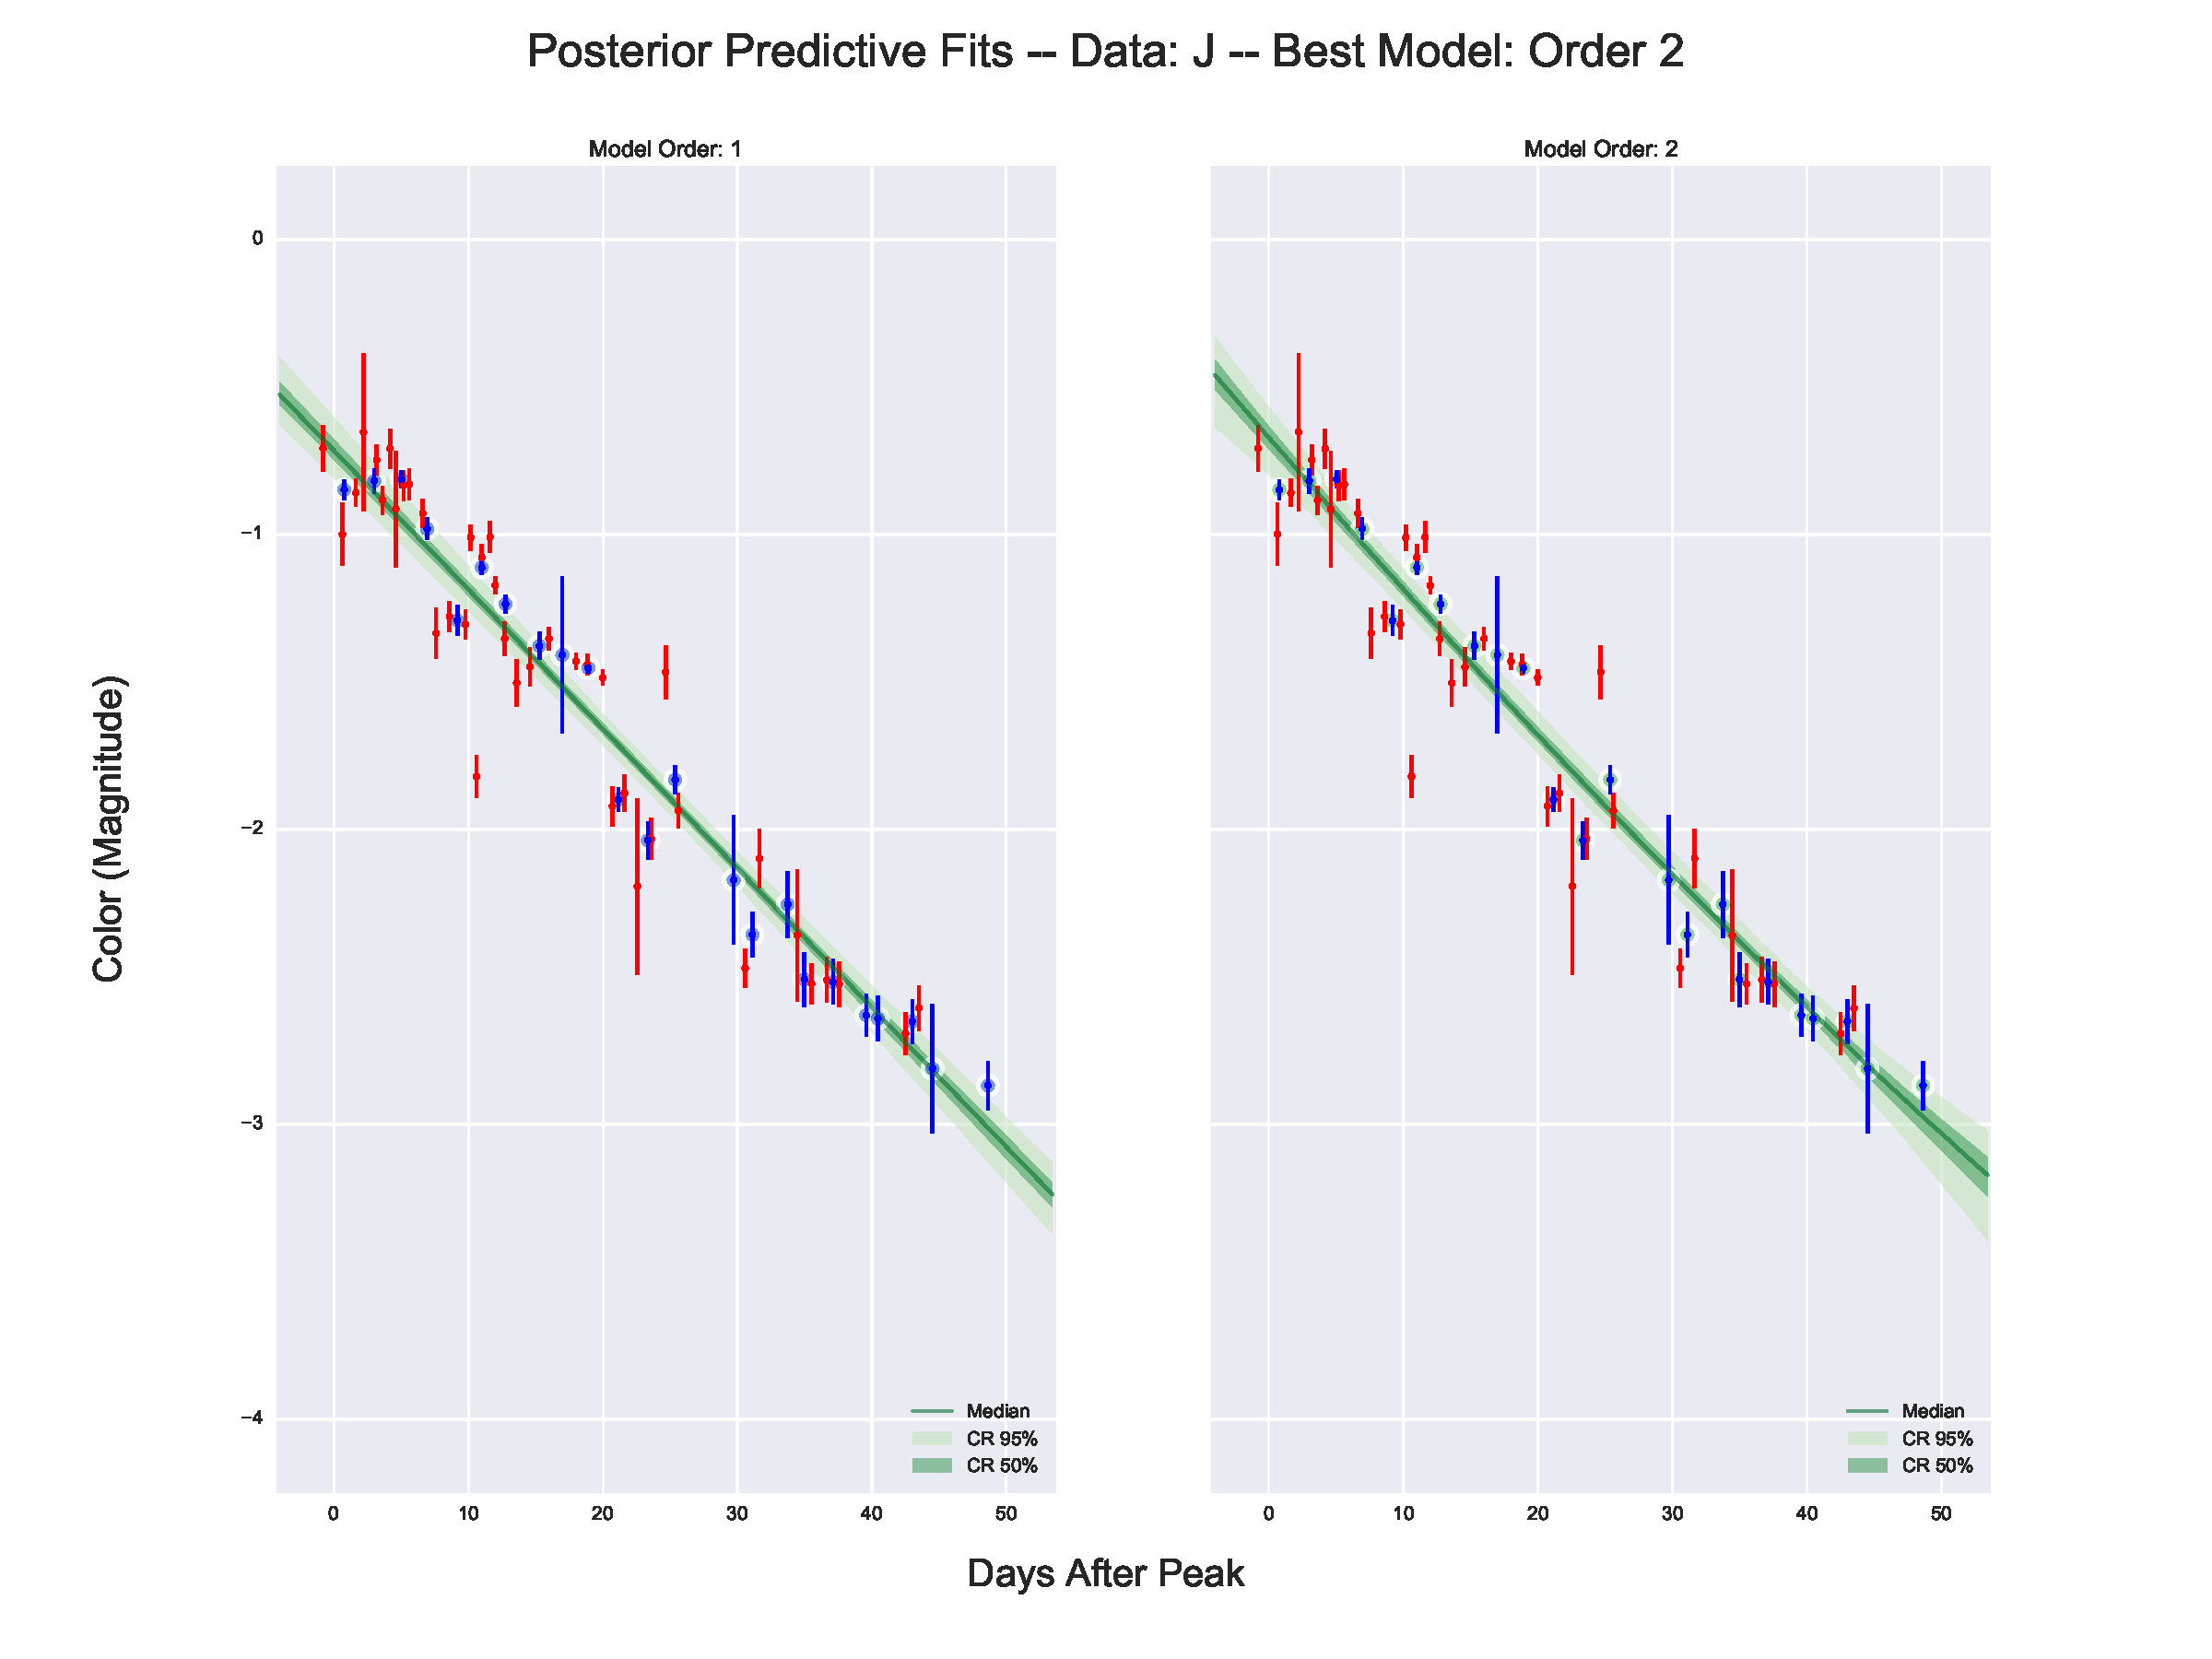
\includegraphics[scale=.5,center]{FIG/type\type/J_fits}
\end{figure}
\begin{figure}[H]
\centering
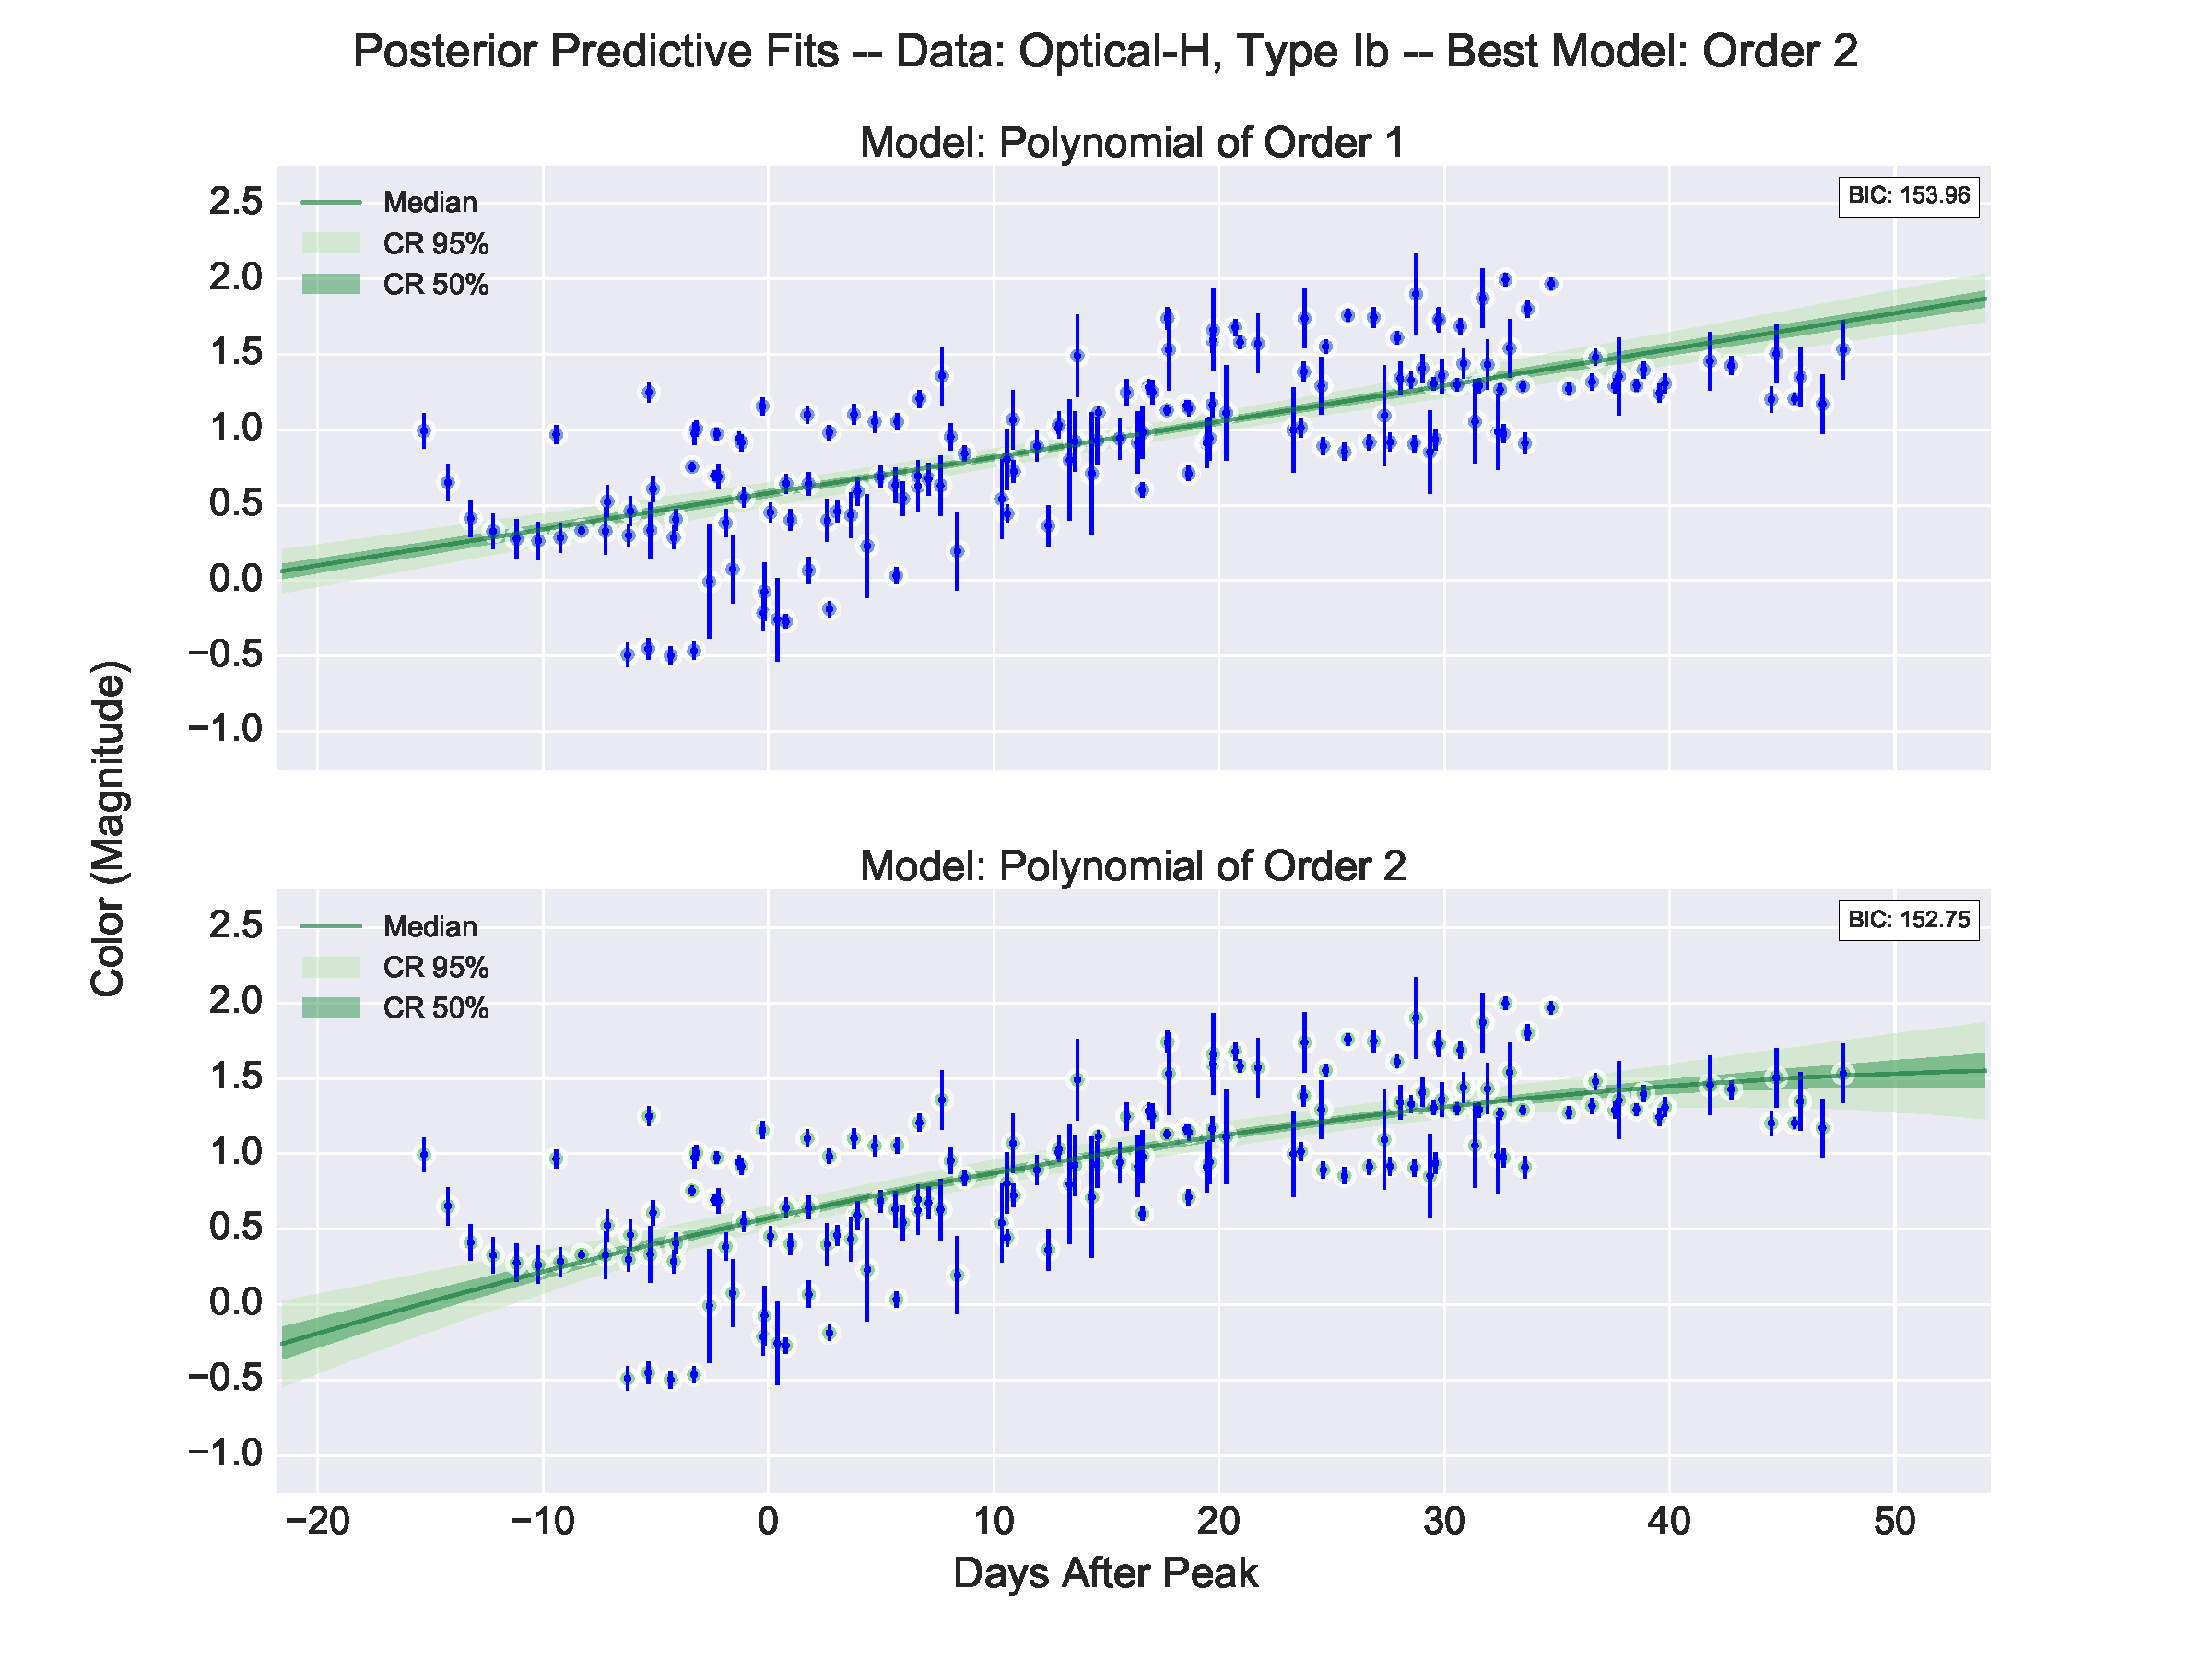
\includegraphics[scale=.5,center]{FIG/type\type/H_fits}
\end{figure}
\begin{figure}[H]
\centering
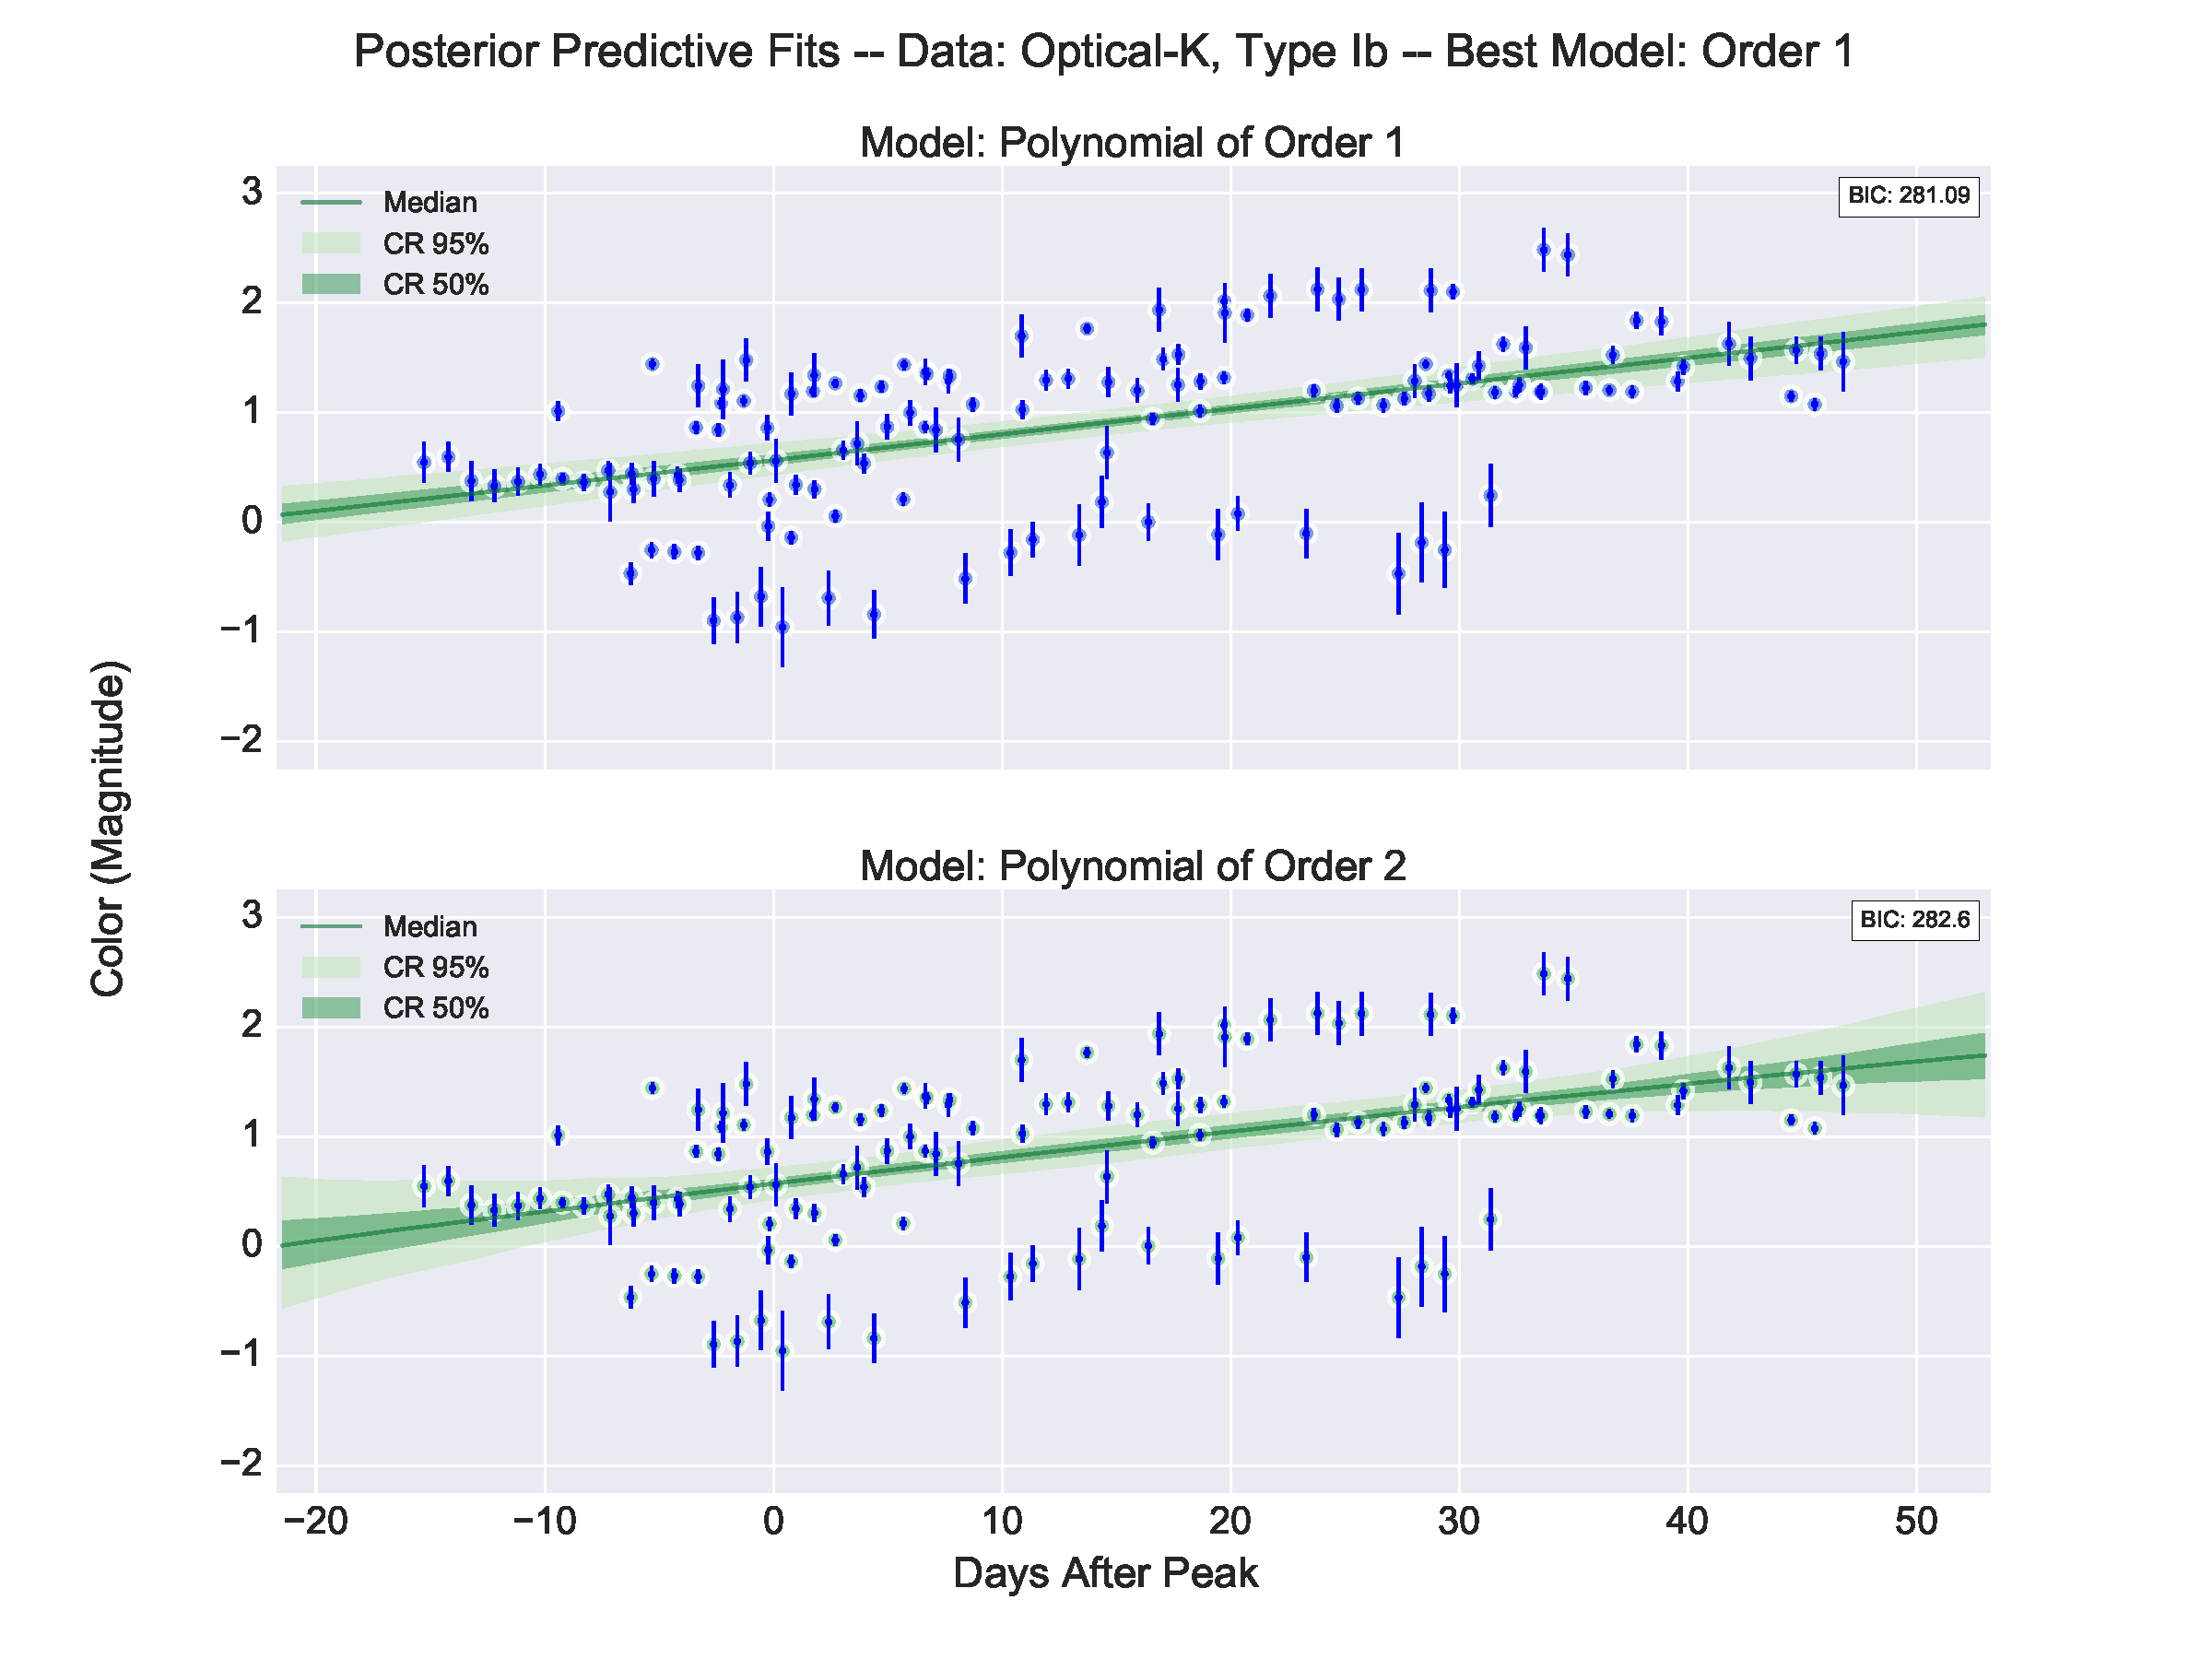
\includegraphics[scale=.5,center]{FIG/type\type/K_fits}
\end{figure}
\begin{figure}[H]
\centering
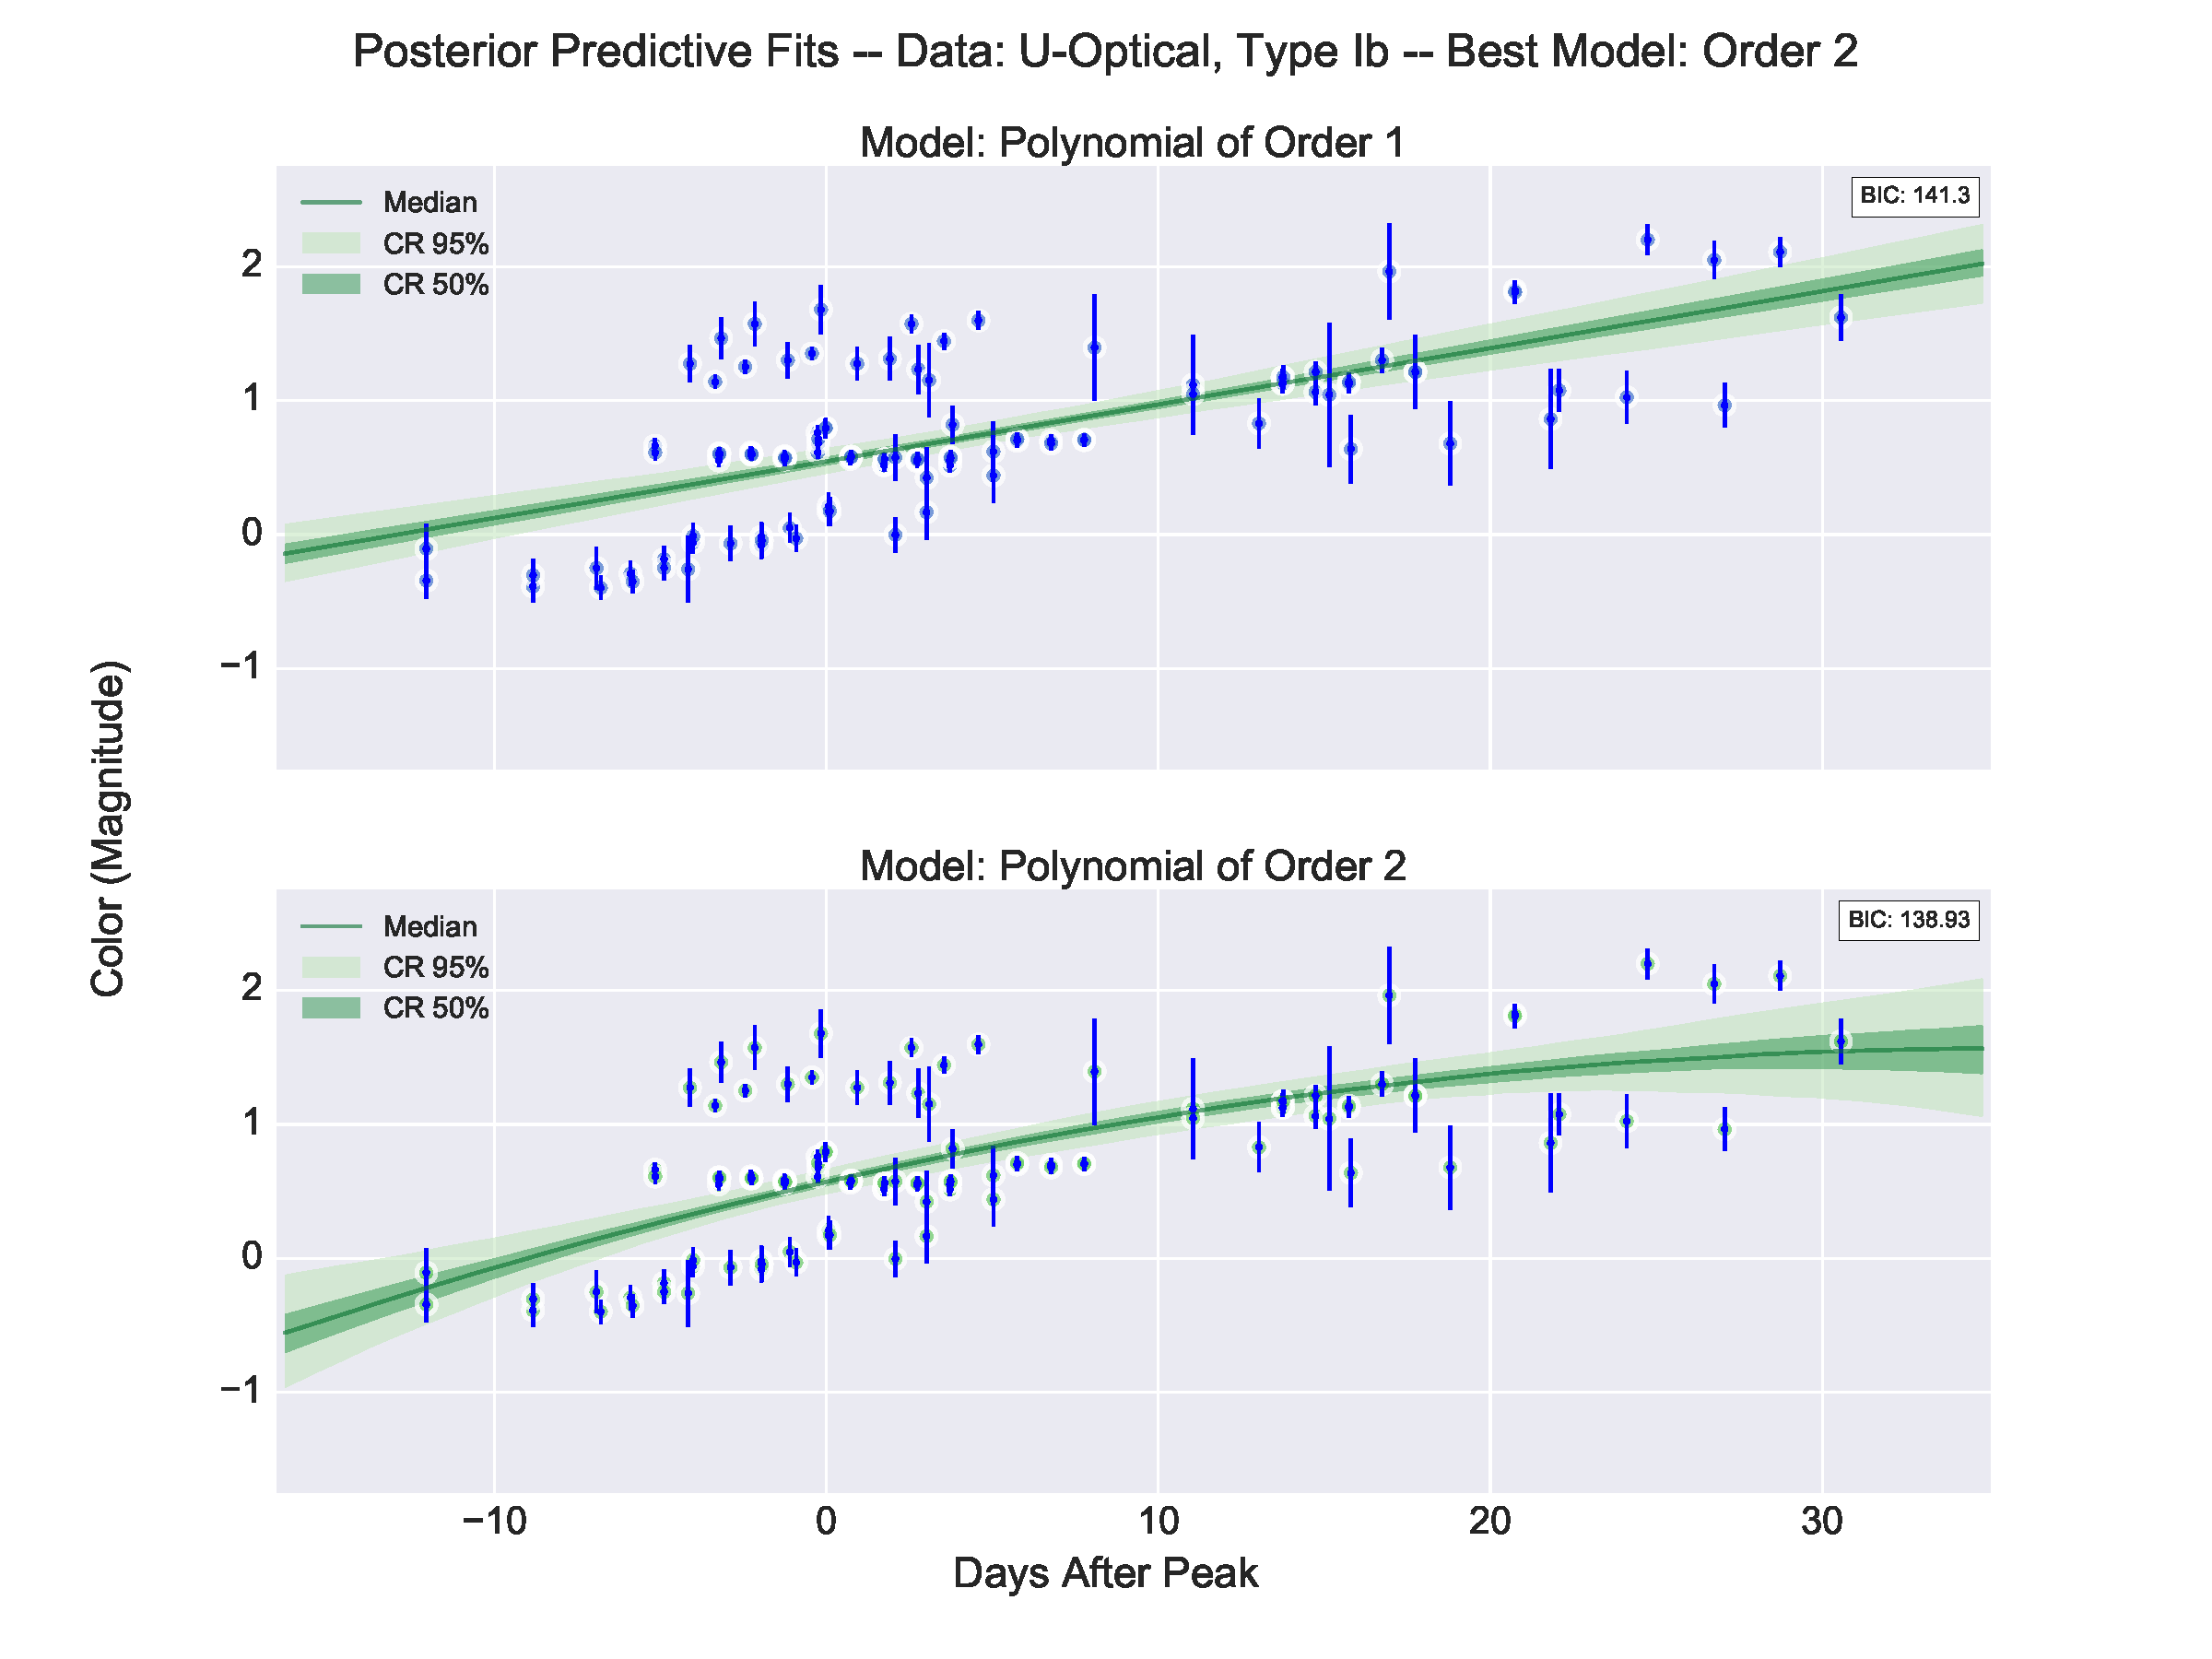
\includegraphics[scale=.5,center]{FIG/type\type/UV_fits}
\end{figure}

\pagebreak
%%Type Ic%%
\renewcommand{\type}{Ic}

\

\textbf{Type \type}
\begin{figure}[H]
%\centering
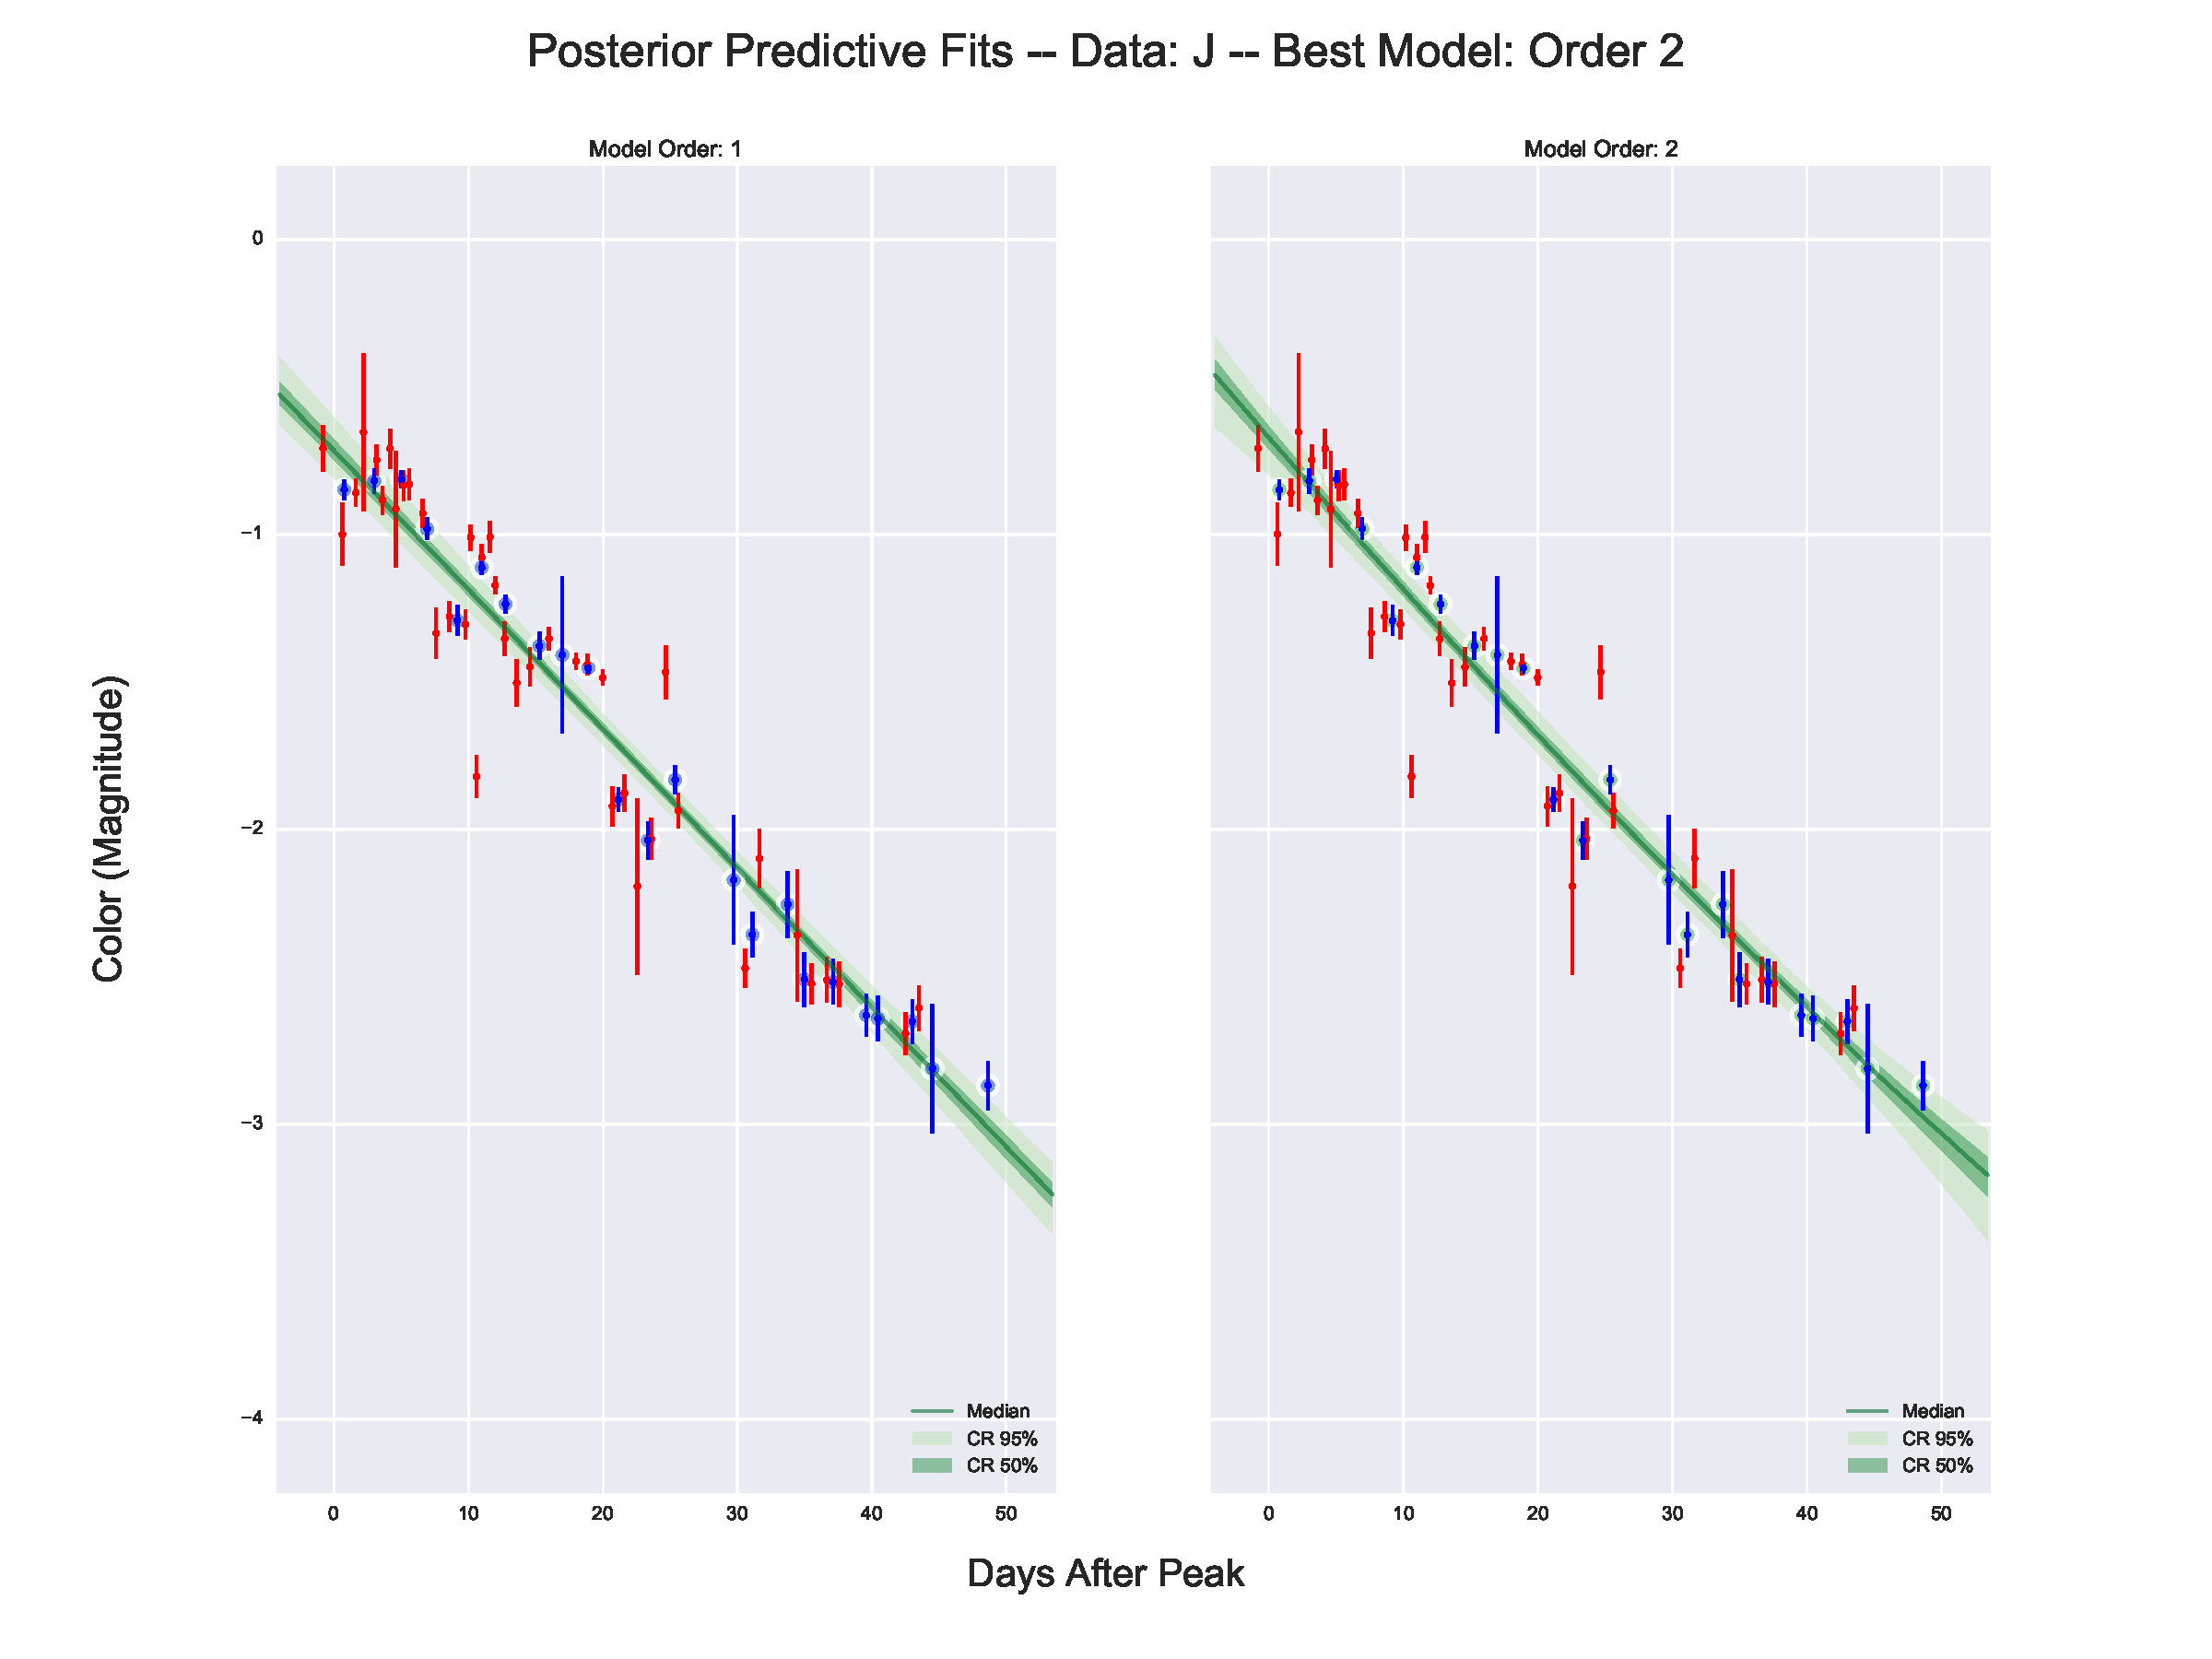
\includegraphics[scale=.5,center]{FIG/type\type/J_fits}
\caption{\label{fig:FIG/typeIb/J_fits} My fig}
\end{figure}
\begin{figure}[H]
\centering
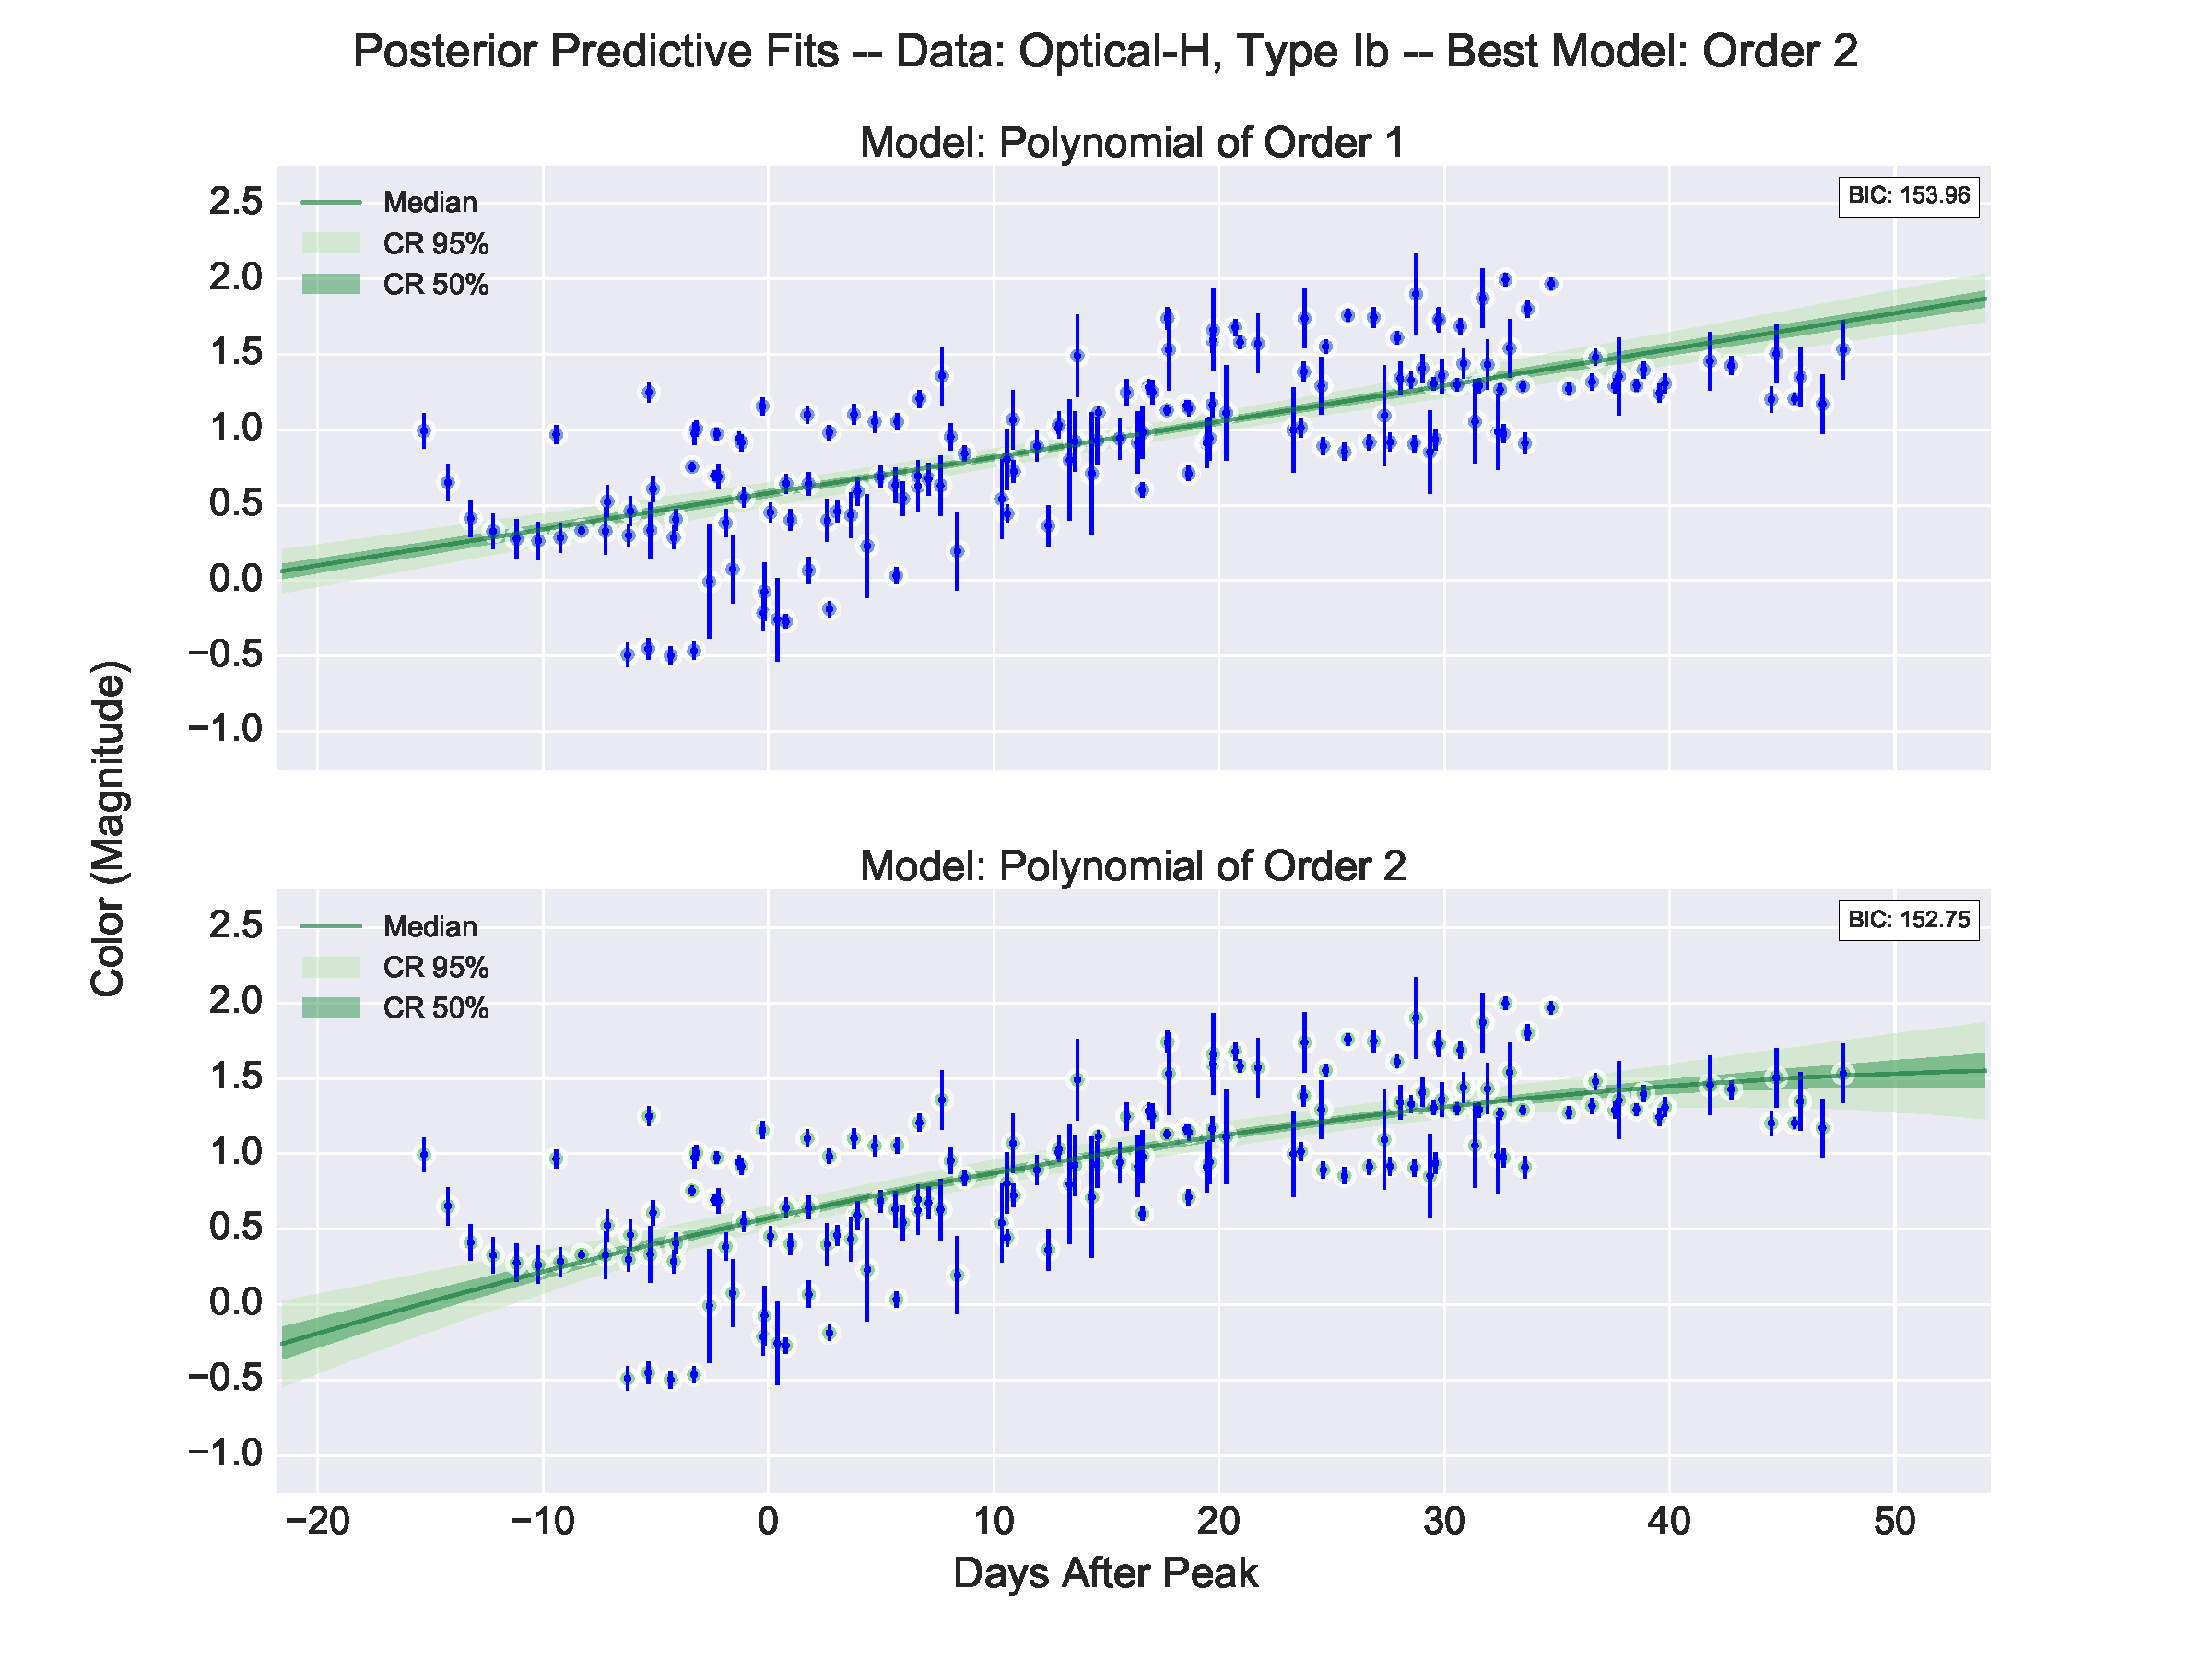
\includegraphics[scale=.5,center]{FIG/type\type/H_fits}
\end{figure}
\begin{figure}[H]
\centering
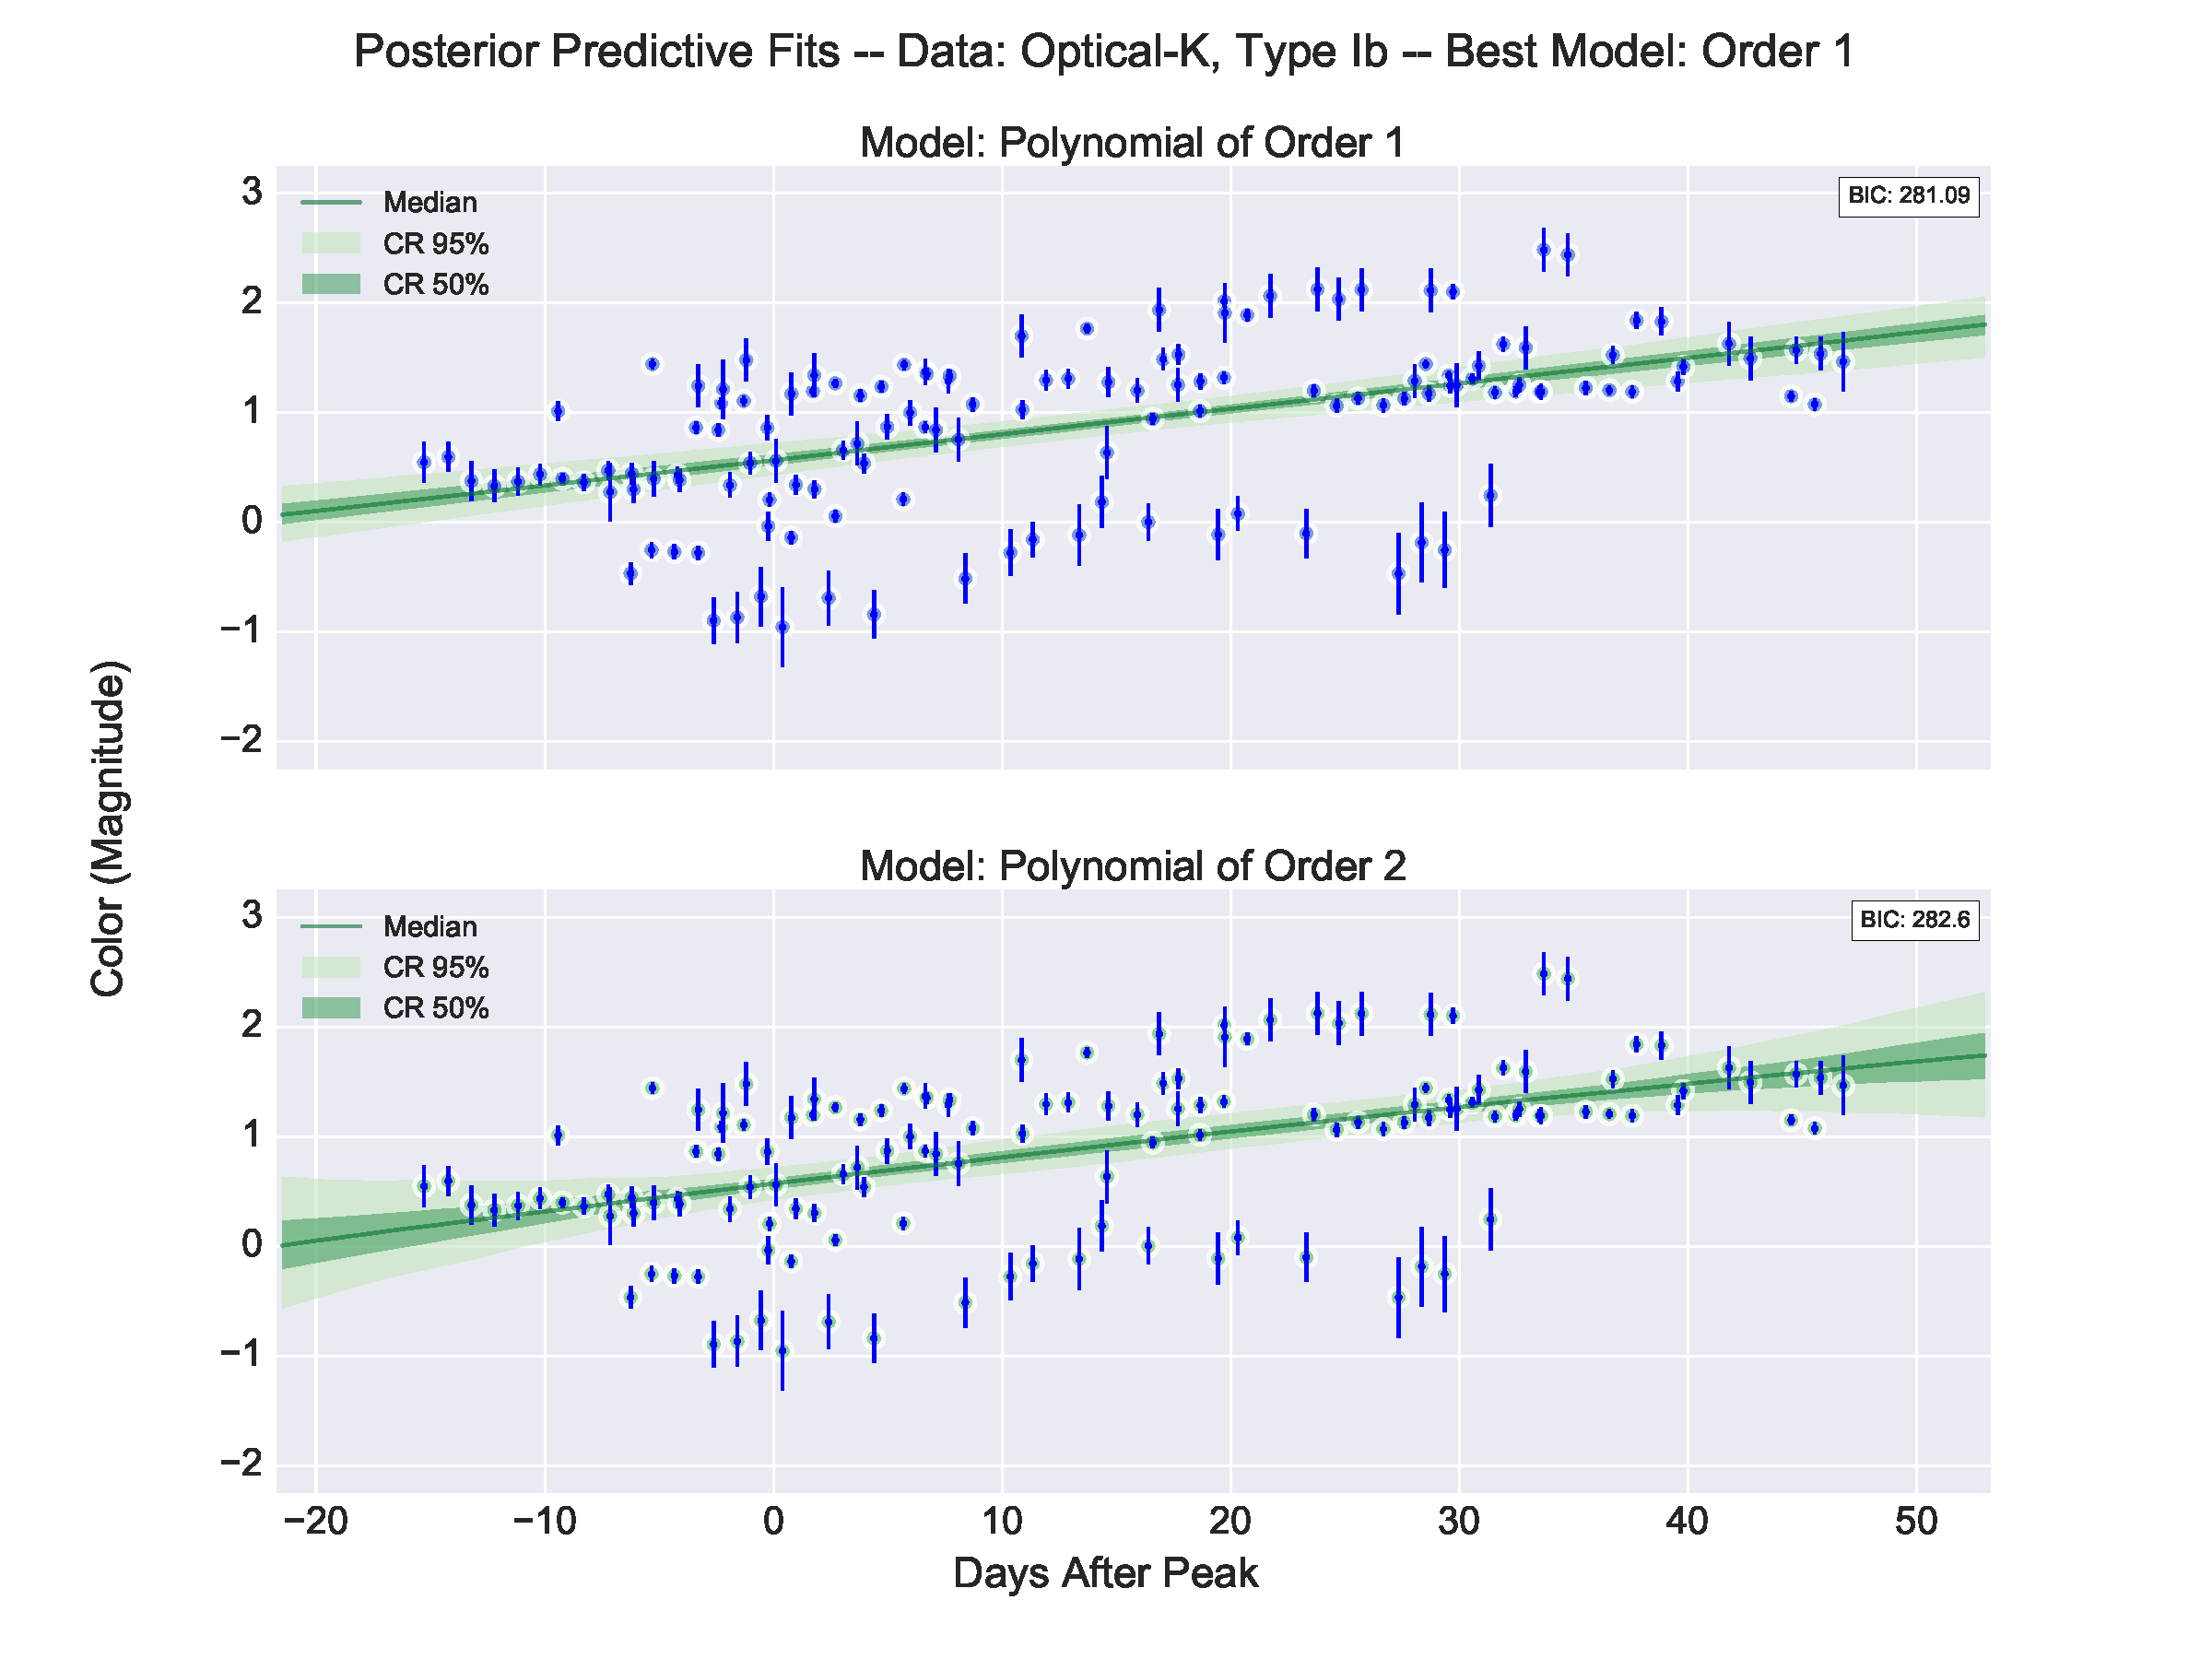
\includegraphics[scale=.5,center]{FIG/type\type/K_fits}
\end{figure}
\begin{figure}[H]
\centering
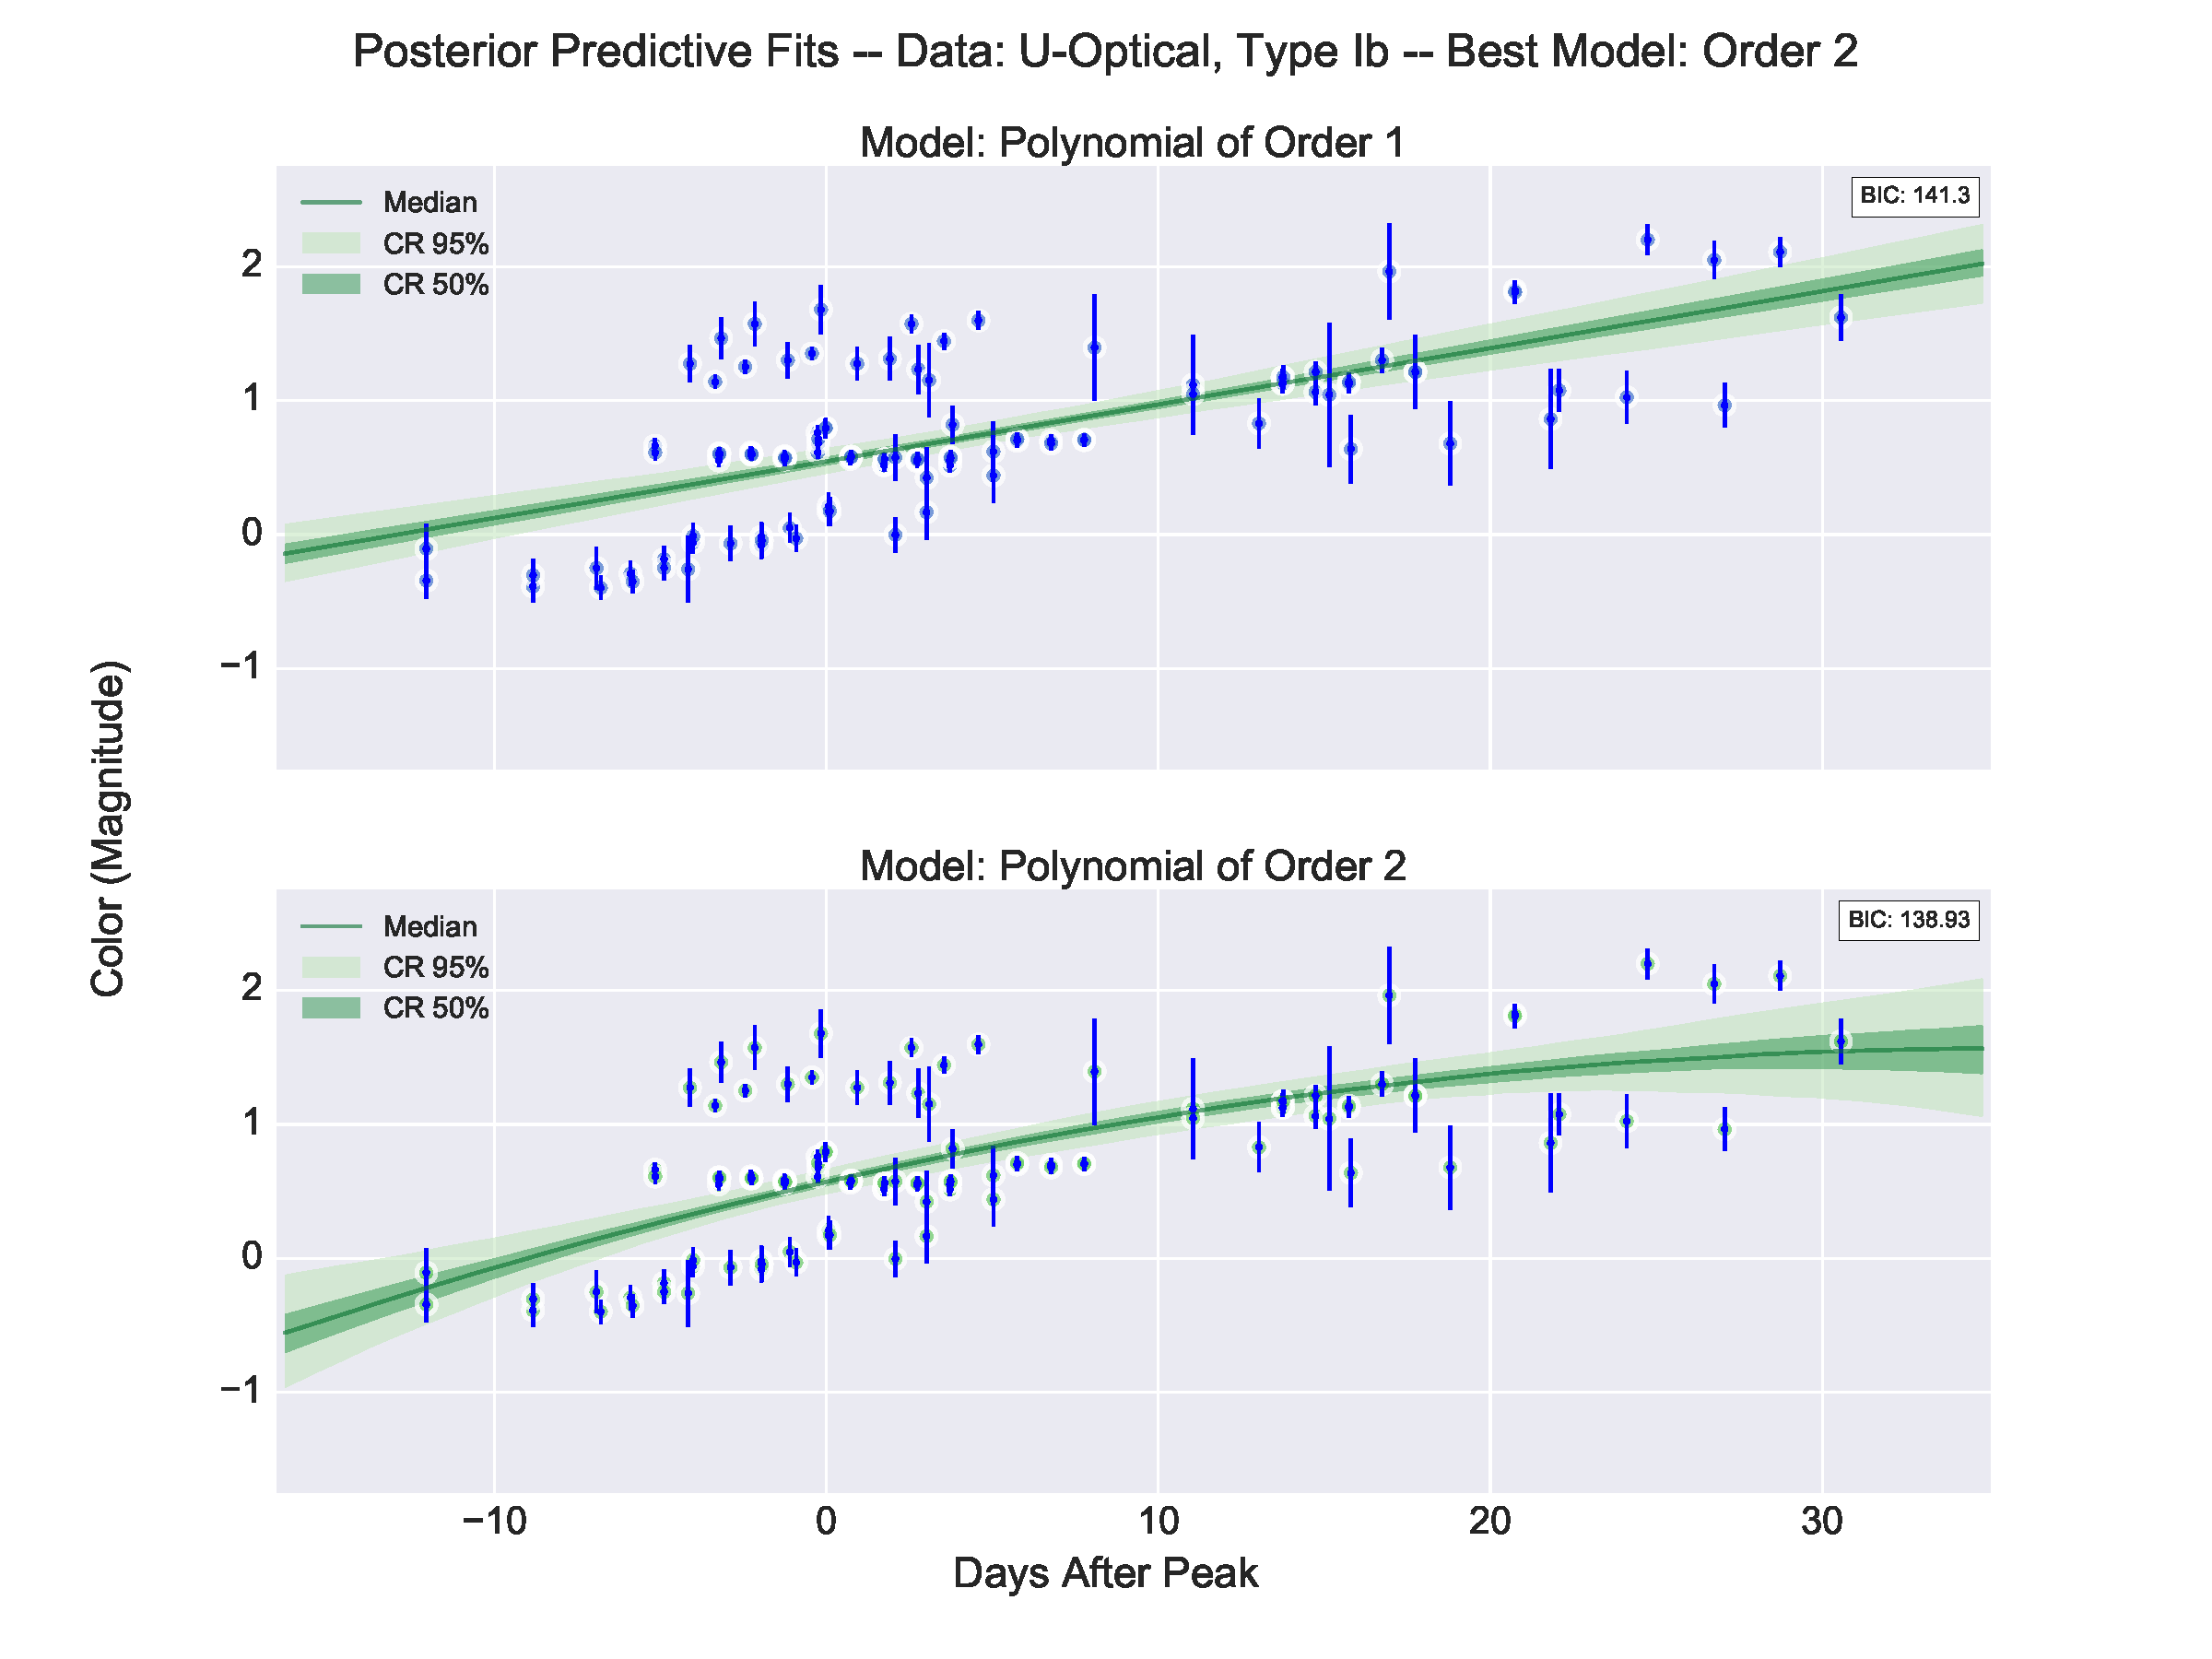
\includegraphics[scale=.5,center]{FIG/type\type/UV_fits}
\end{figure}
\pagebreak
%%Type II+IIP%%
\renewcommand{\type}{II}
\textbf{Type \type + IIP}
\begin{figure}[H]
%\centering
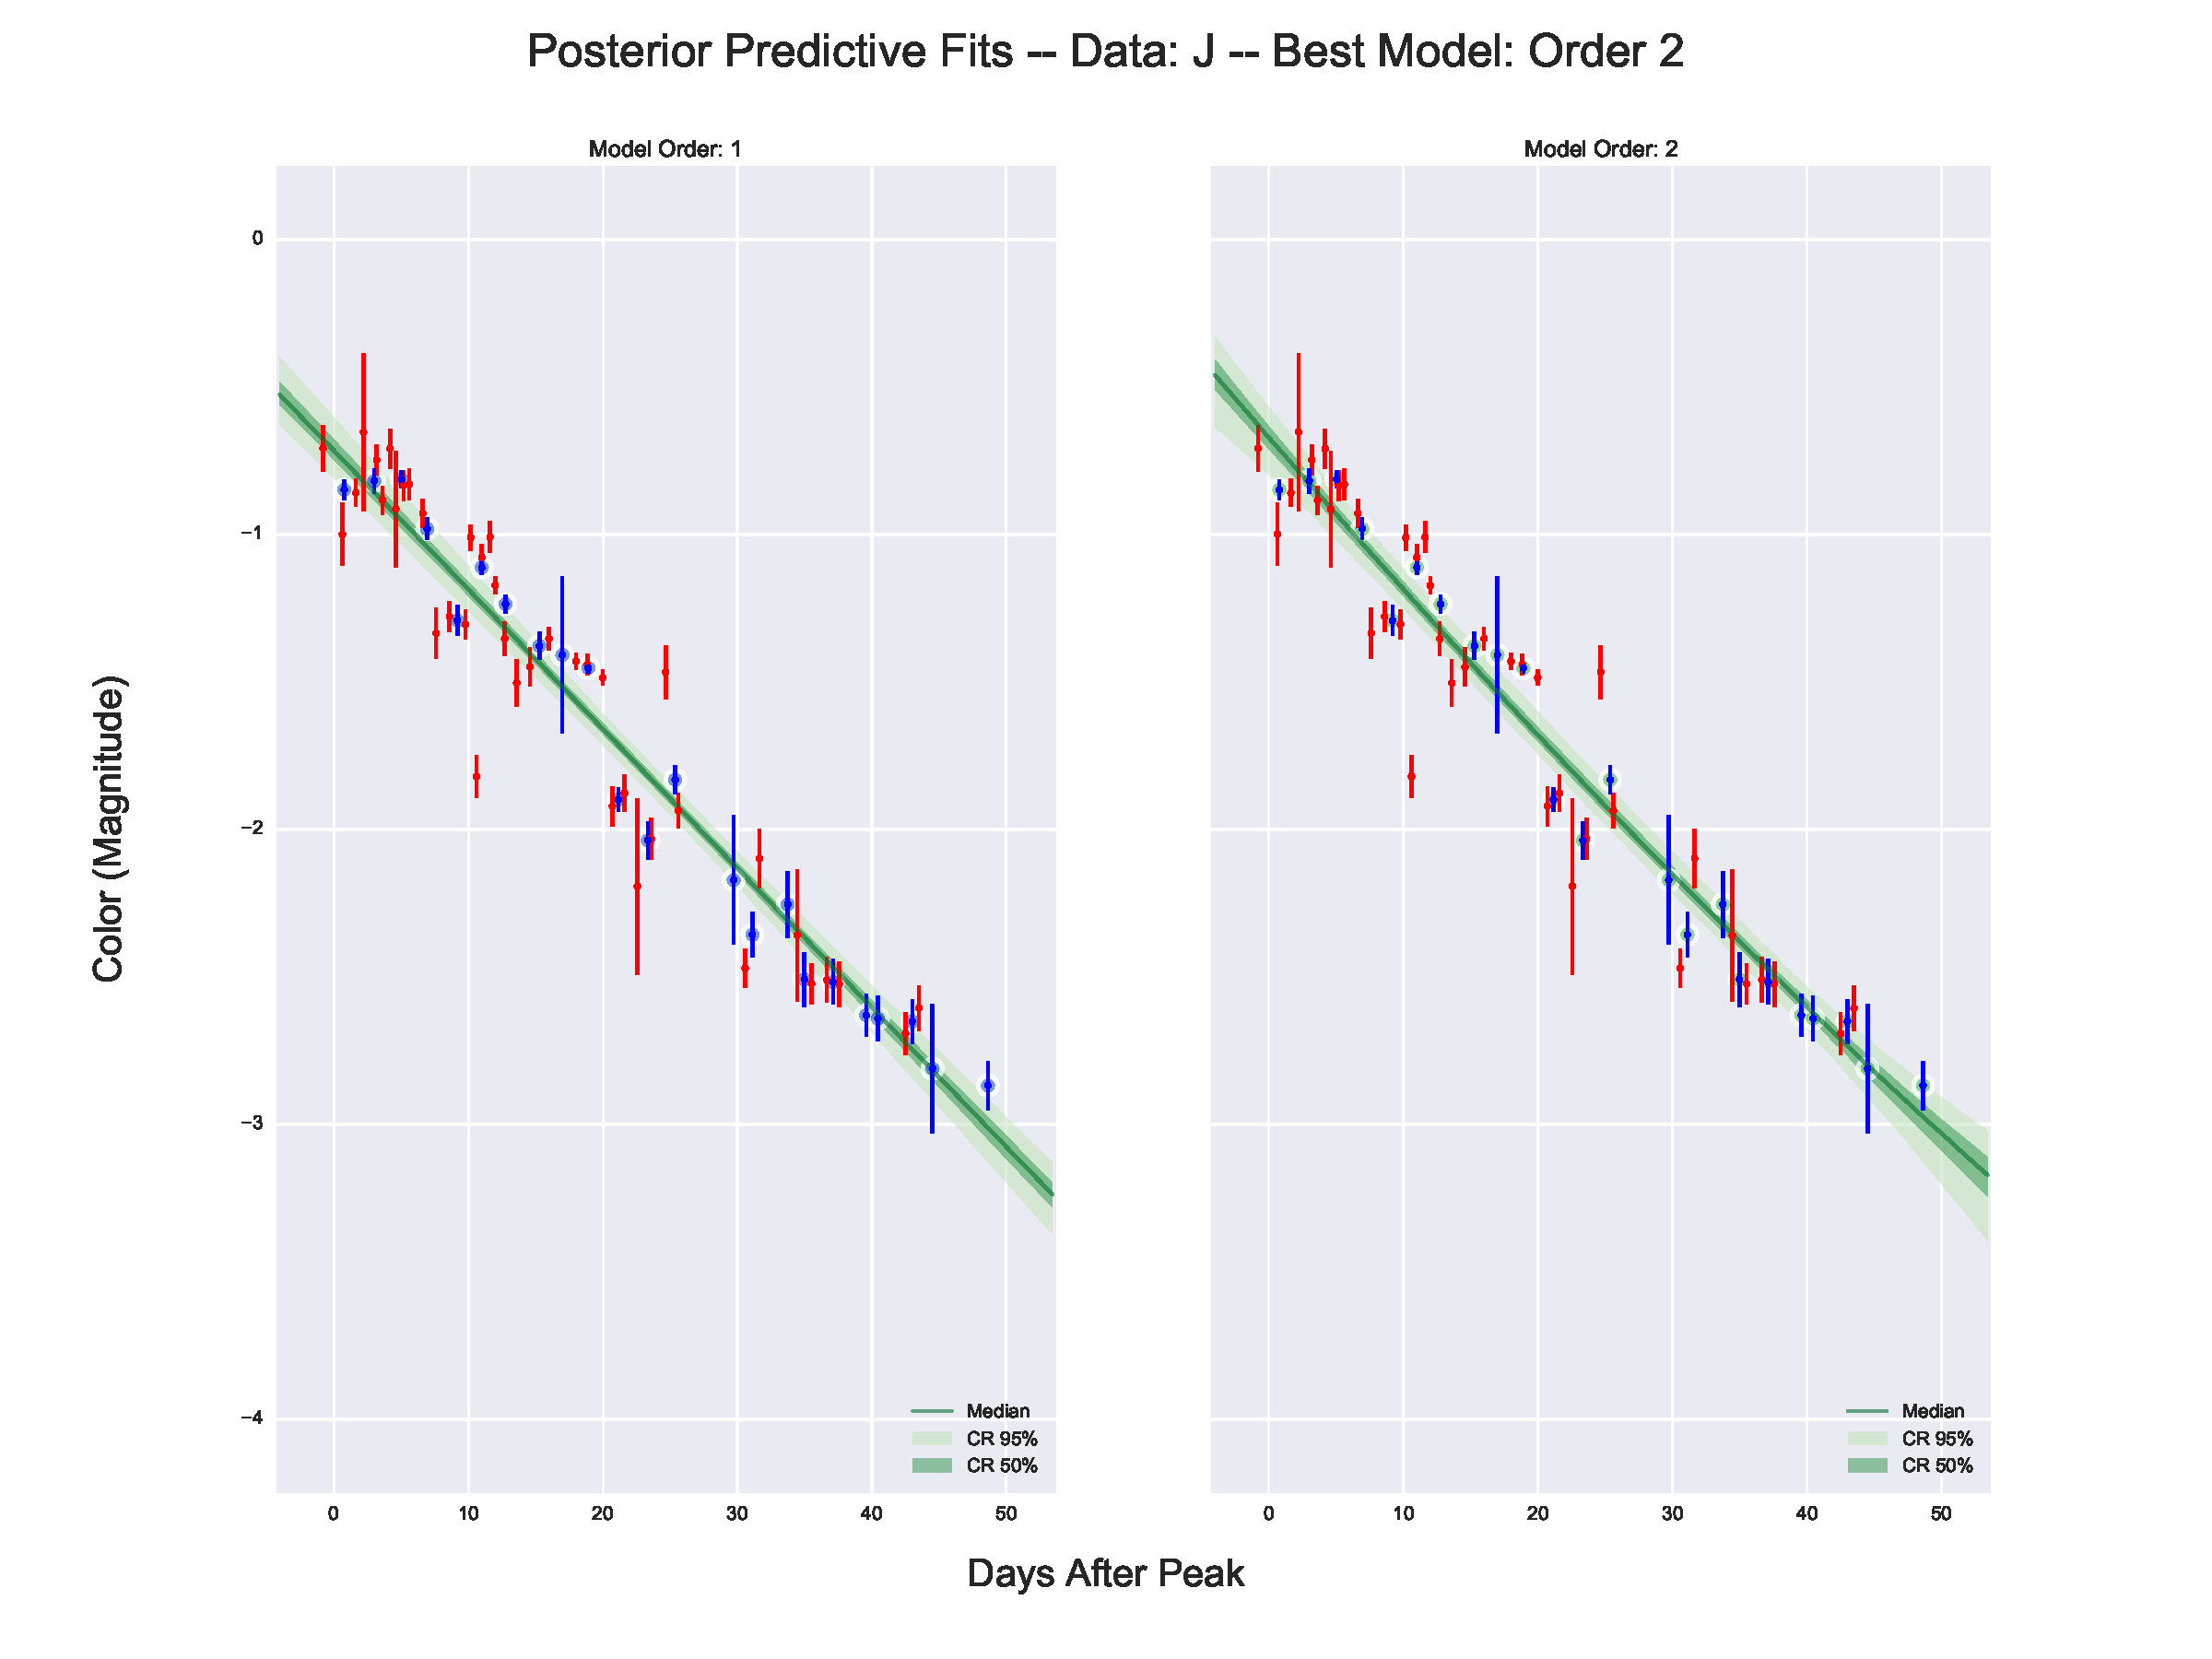
\includegraphics[scale=.5,center]{FIG/type\type/J_fits}
\caption{\label{fig:FIG/typeIb/J_fits} My fig}
\end{figure}
\begin{figure}[H]
\centering
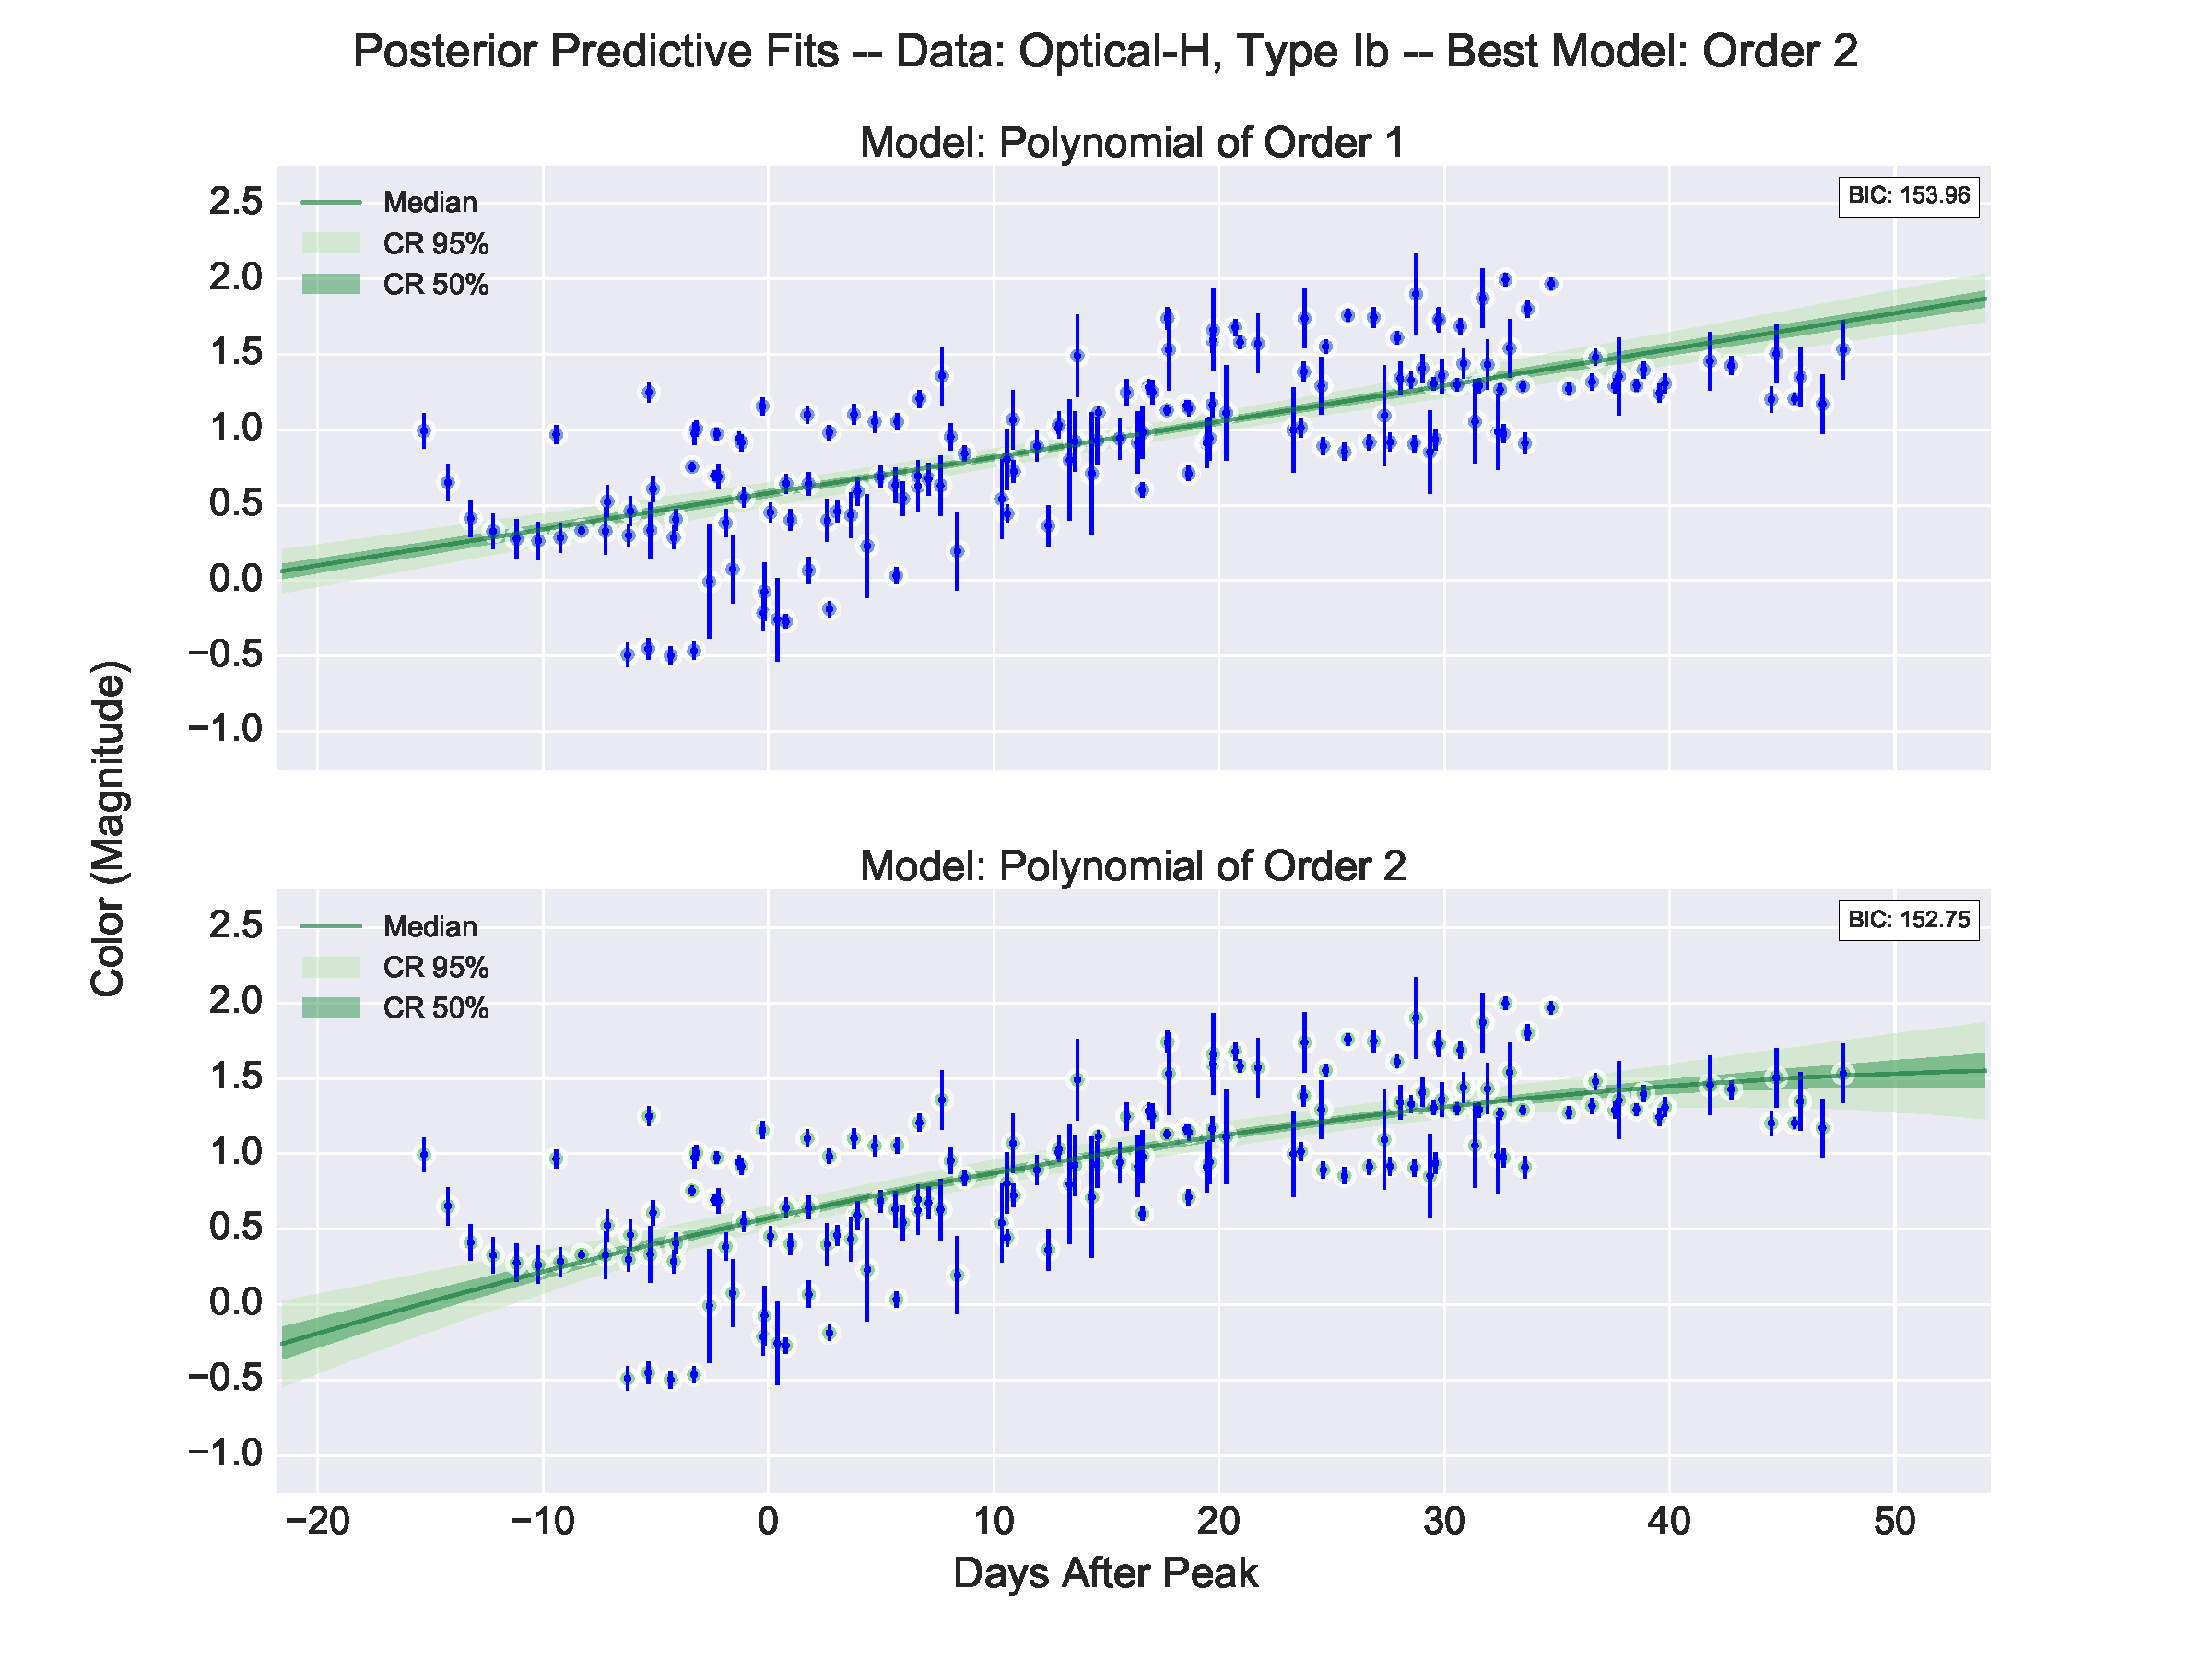
\includegraphics[scale=.5,center]{FIG/type\type/H_fits}
\end{figure}
\begin{figure}[H]
\centering
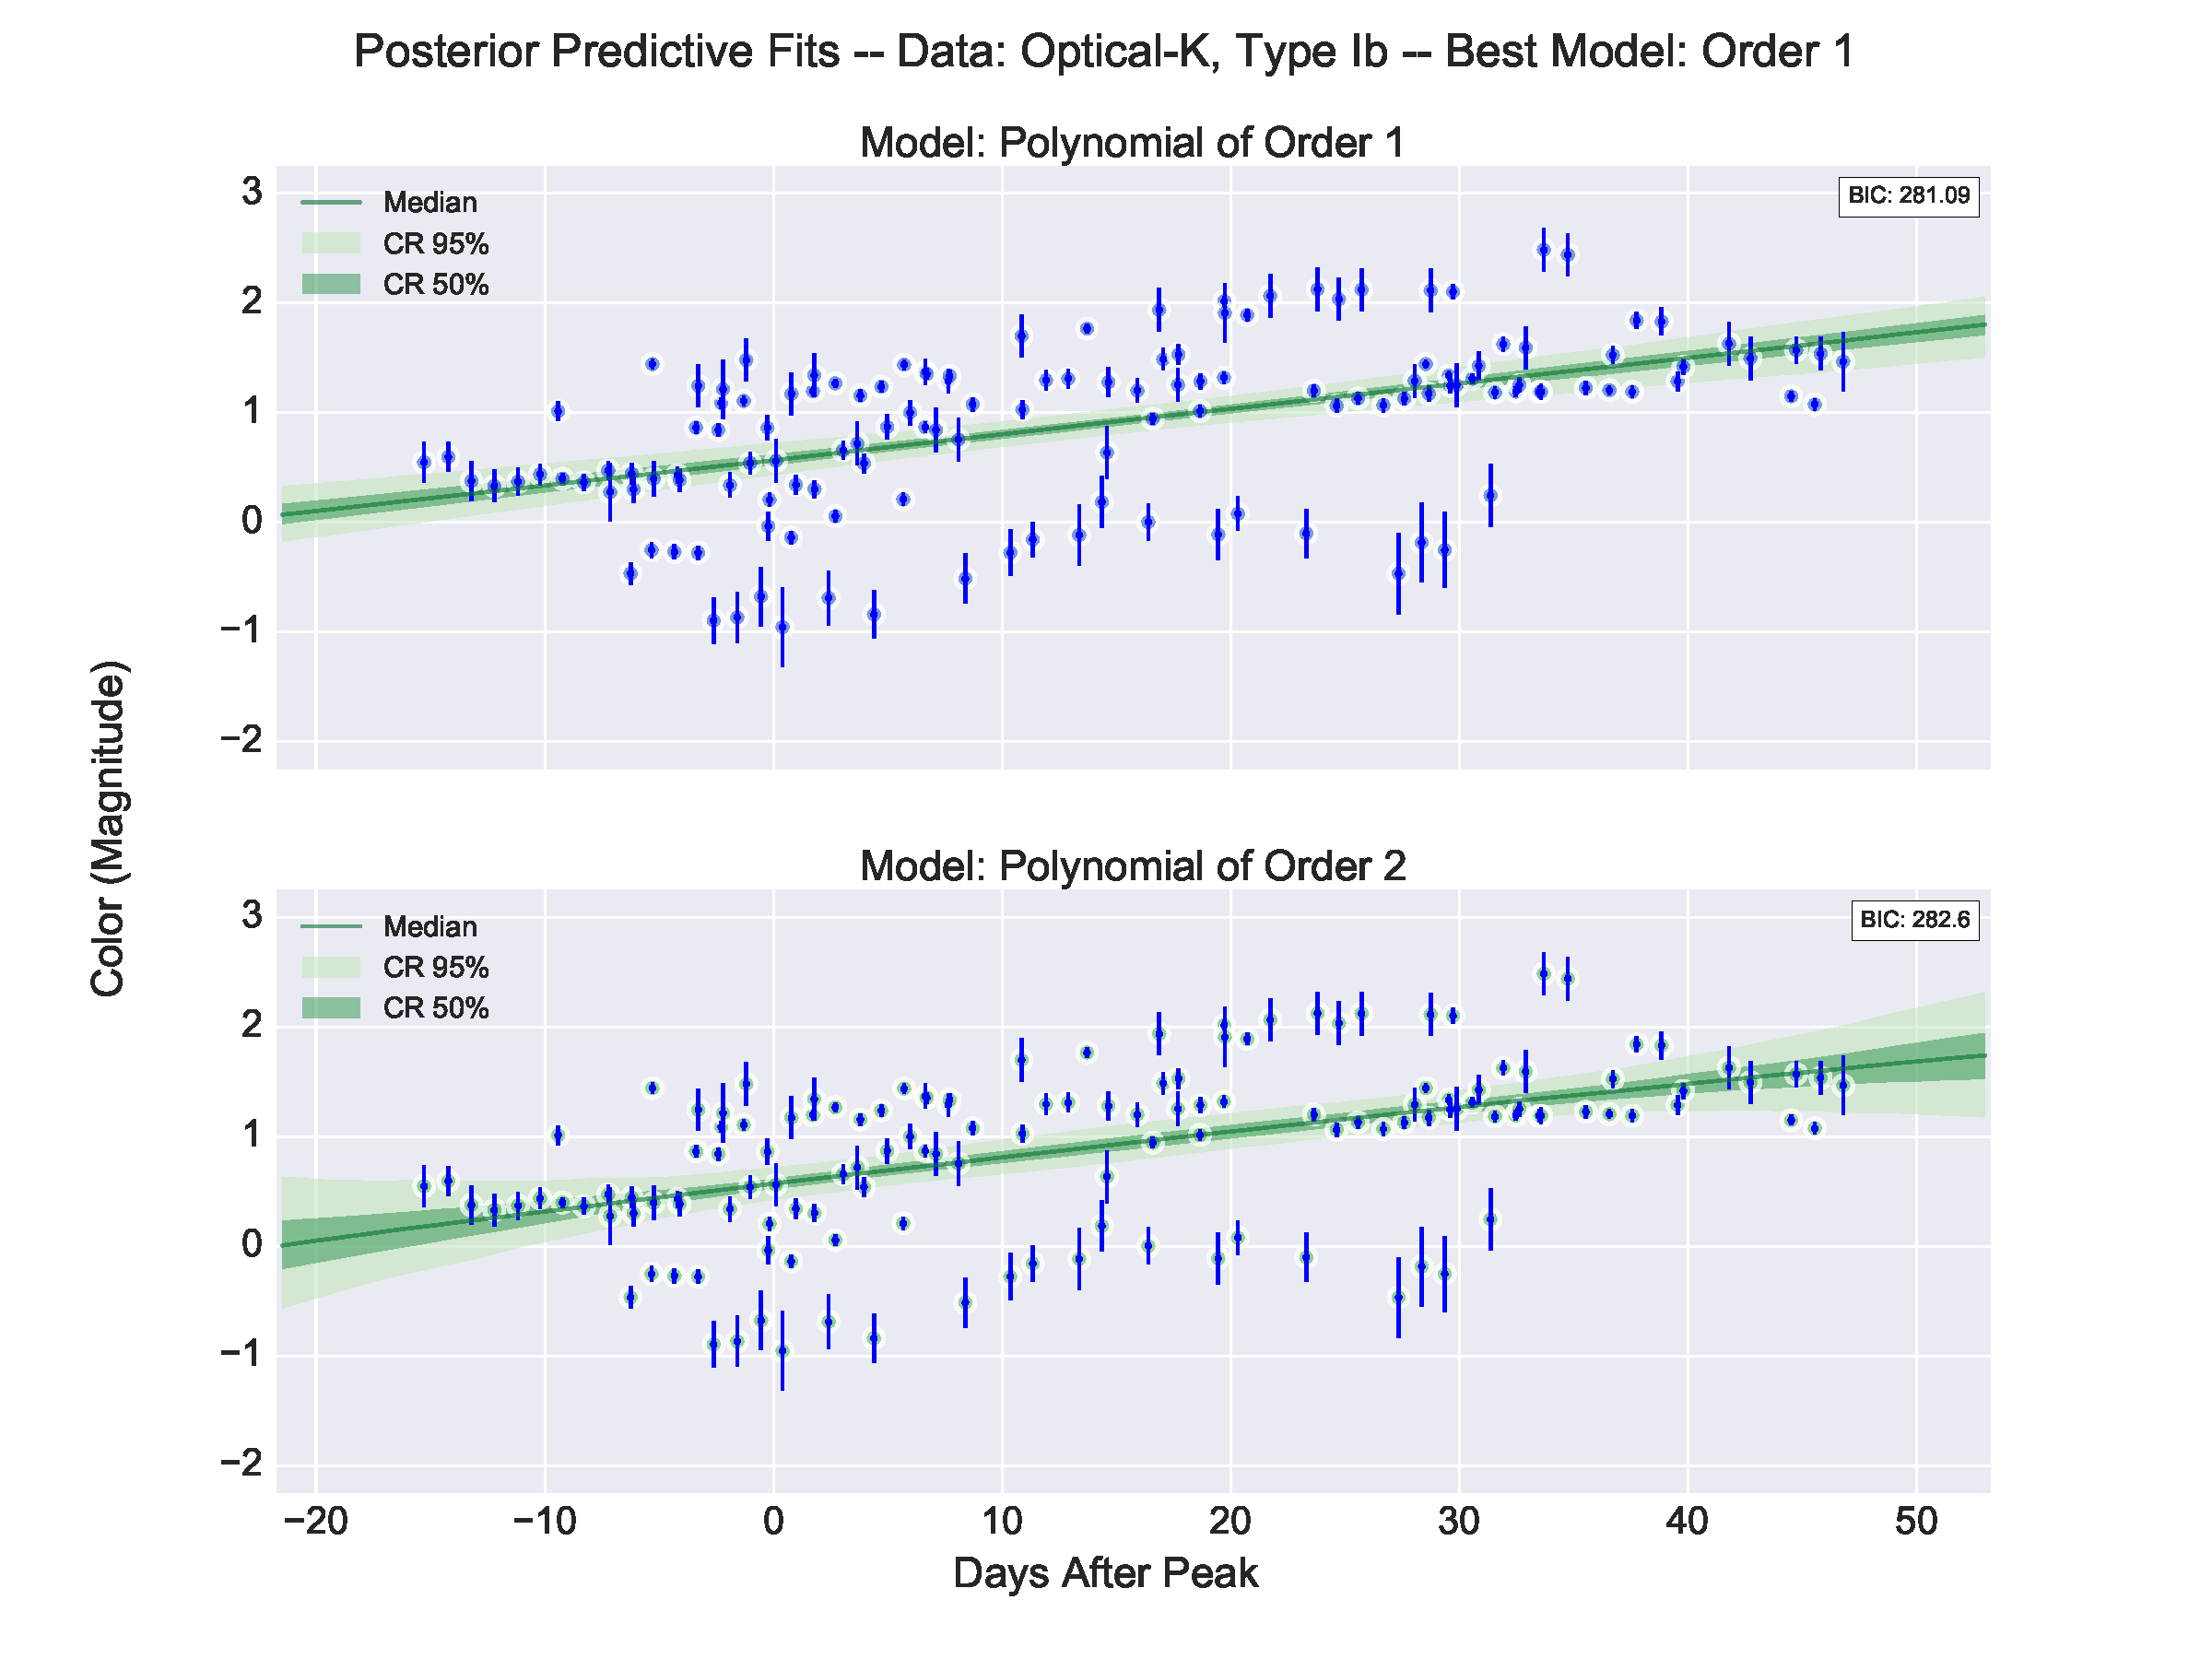
\includegraphics[scale=.5,center]{FIG/type\type/K_fits}
\end{figure}
\begin{figure}[H]
\centering
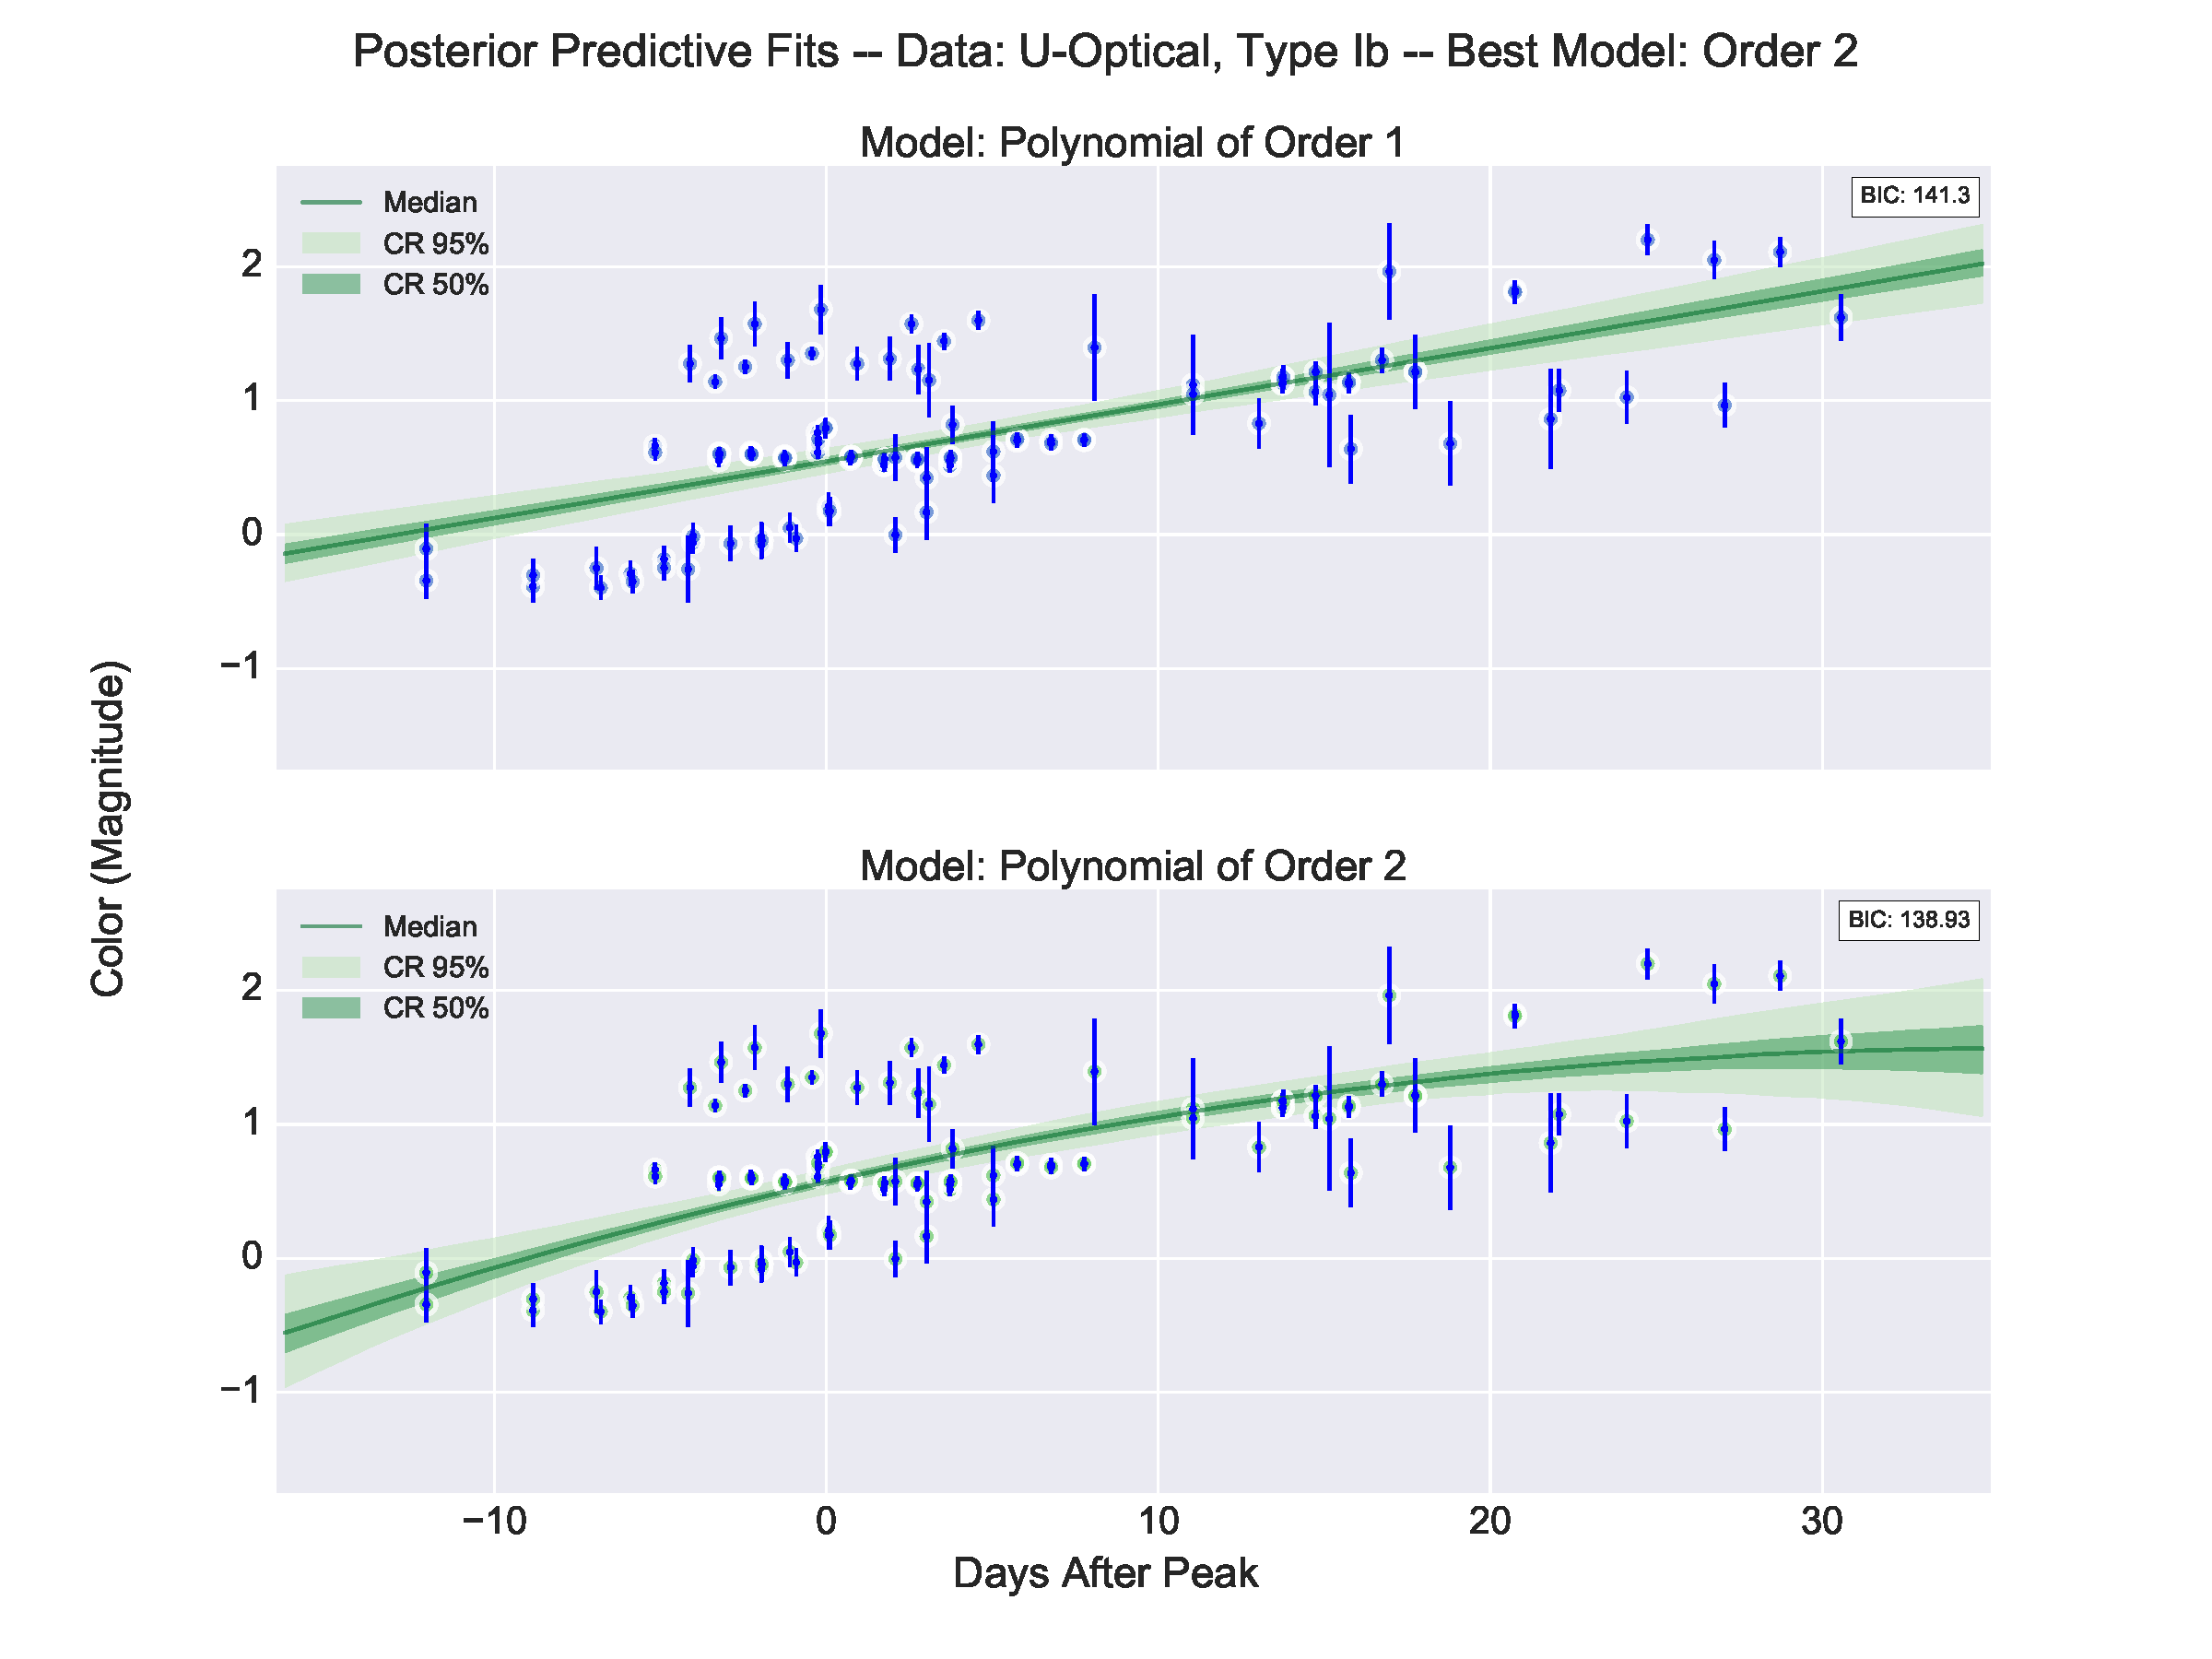
\includegraphics[scale=.5,center]{FIG/type\type/UV_fits}
\end{figure}
\pagebreak

\renewcommand{\type}{IIn}
\textbf{Type \type}
\begin{figure}[H]
%\centering
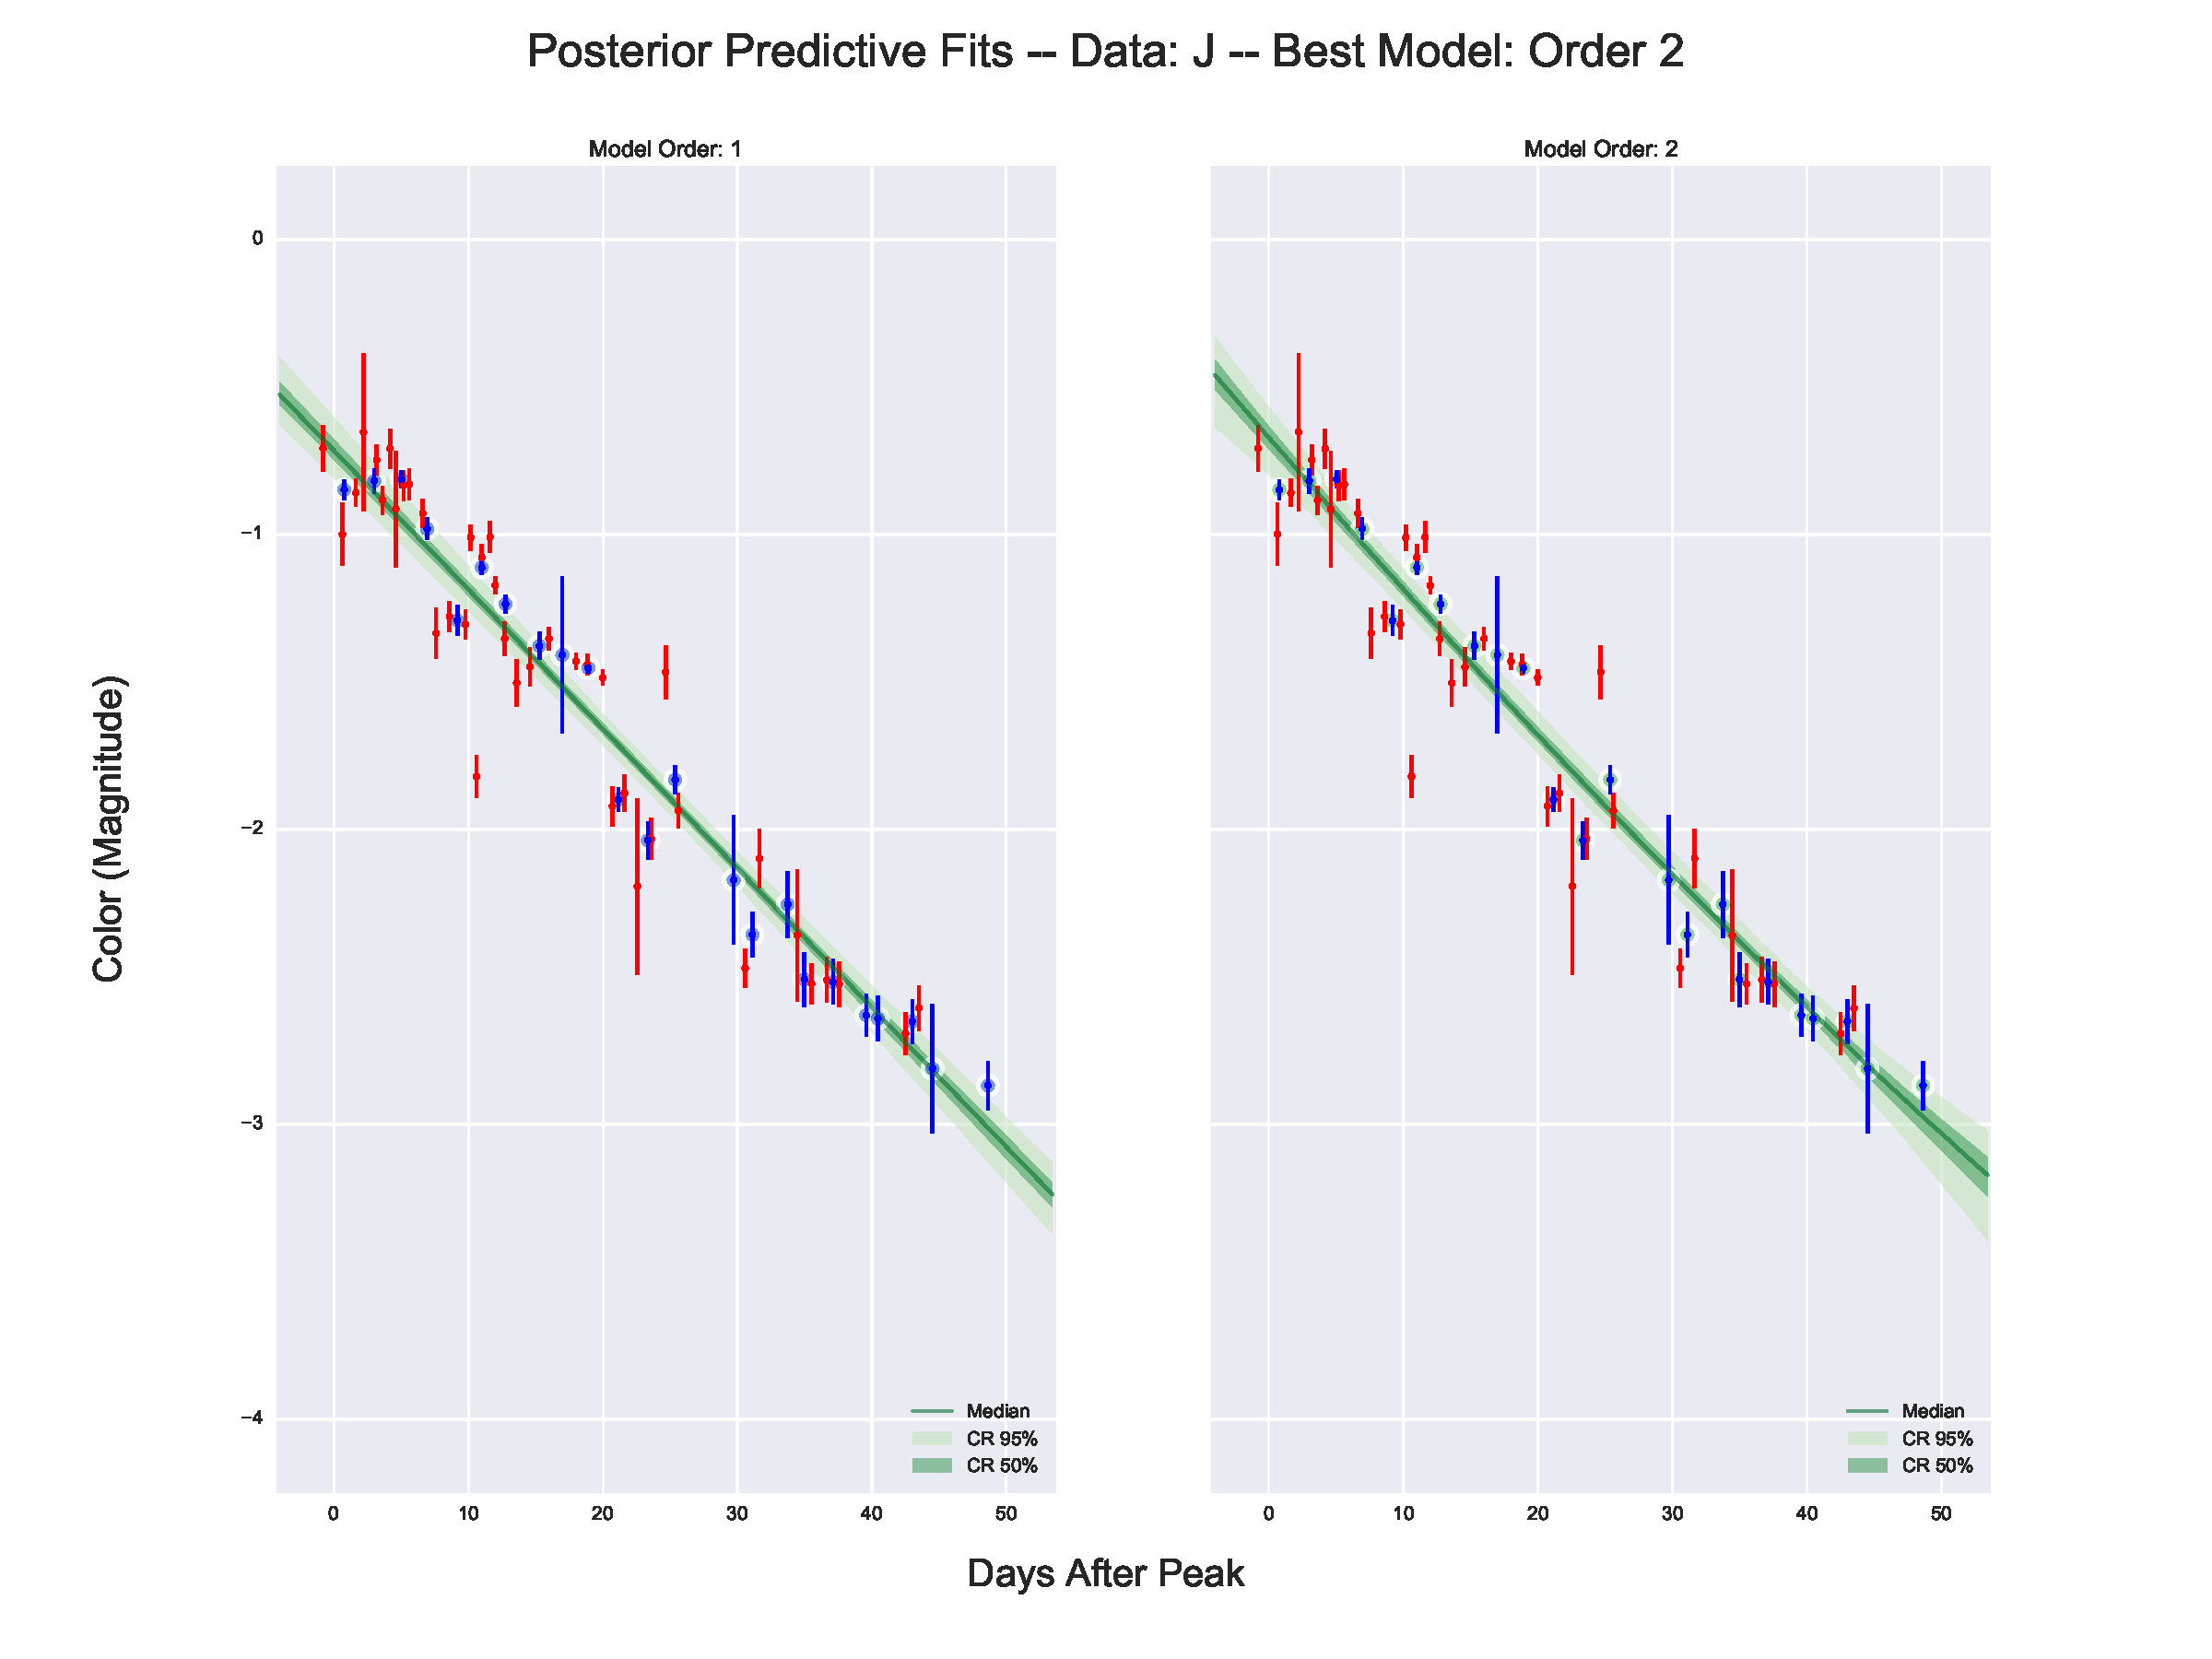
\includegraphics[scale=.5,center]{FIG/type\type/J_fits}
\caption{\label{fig:FIG/typeIb/J_fits} My fig}
\end{figure}
\begin{figure}[H]
\centering
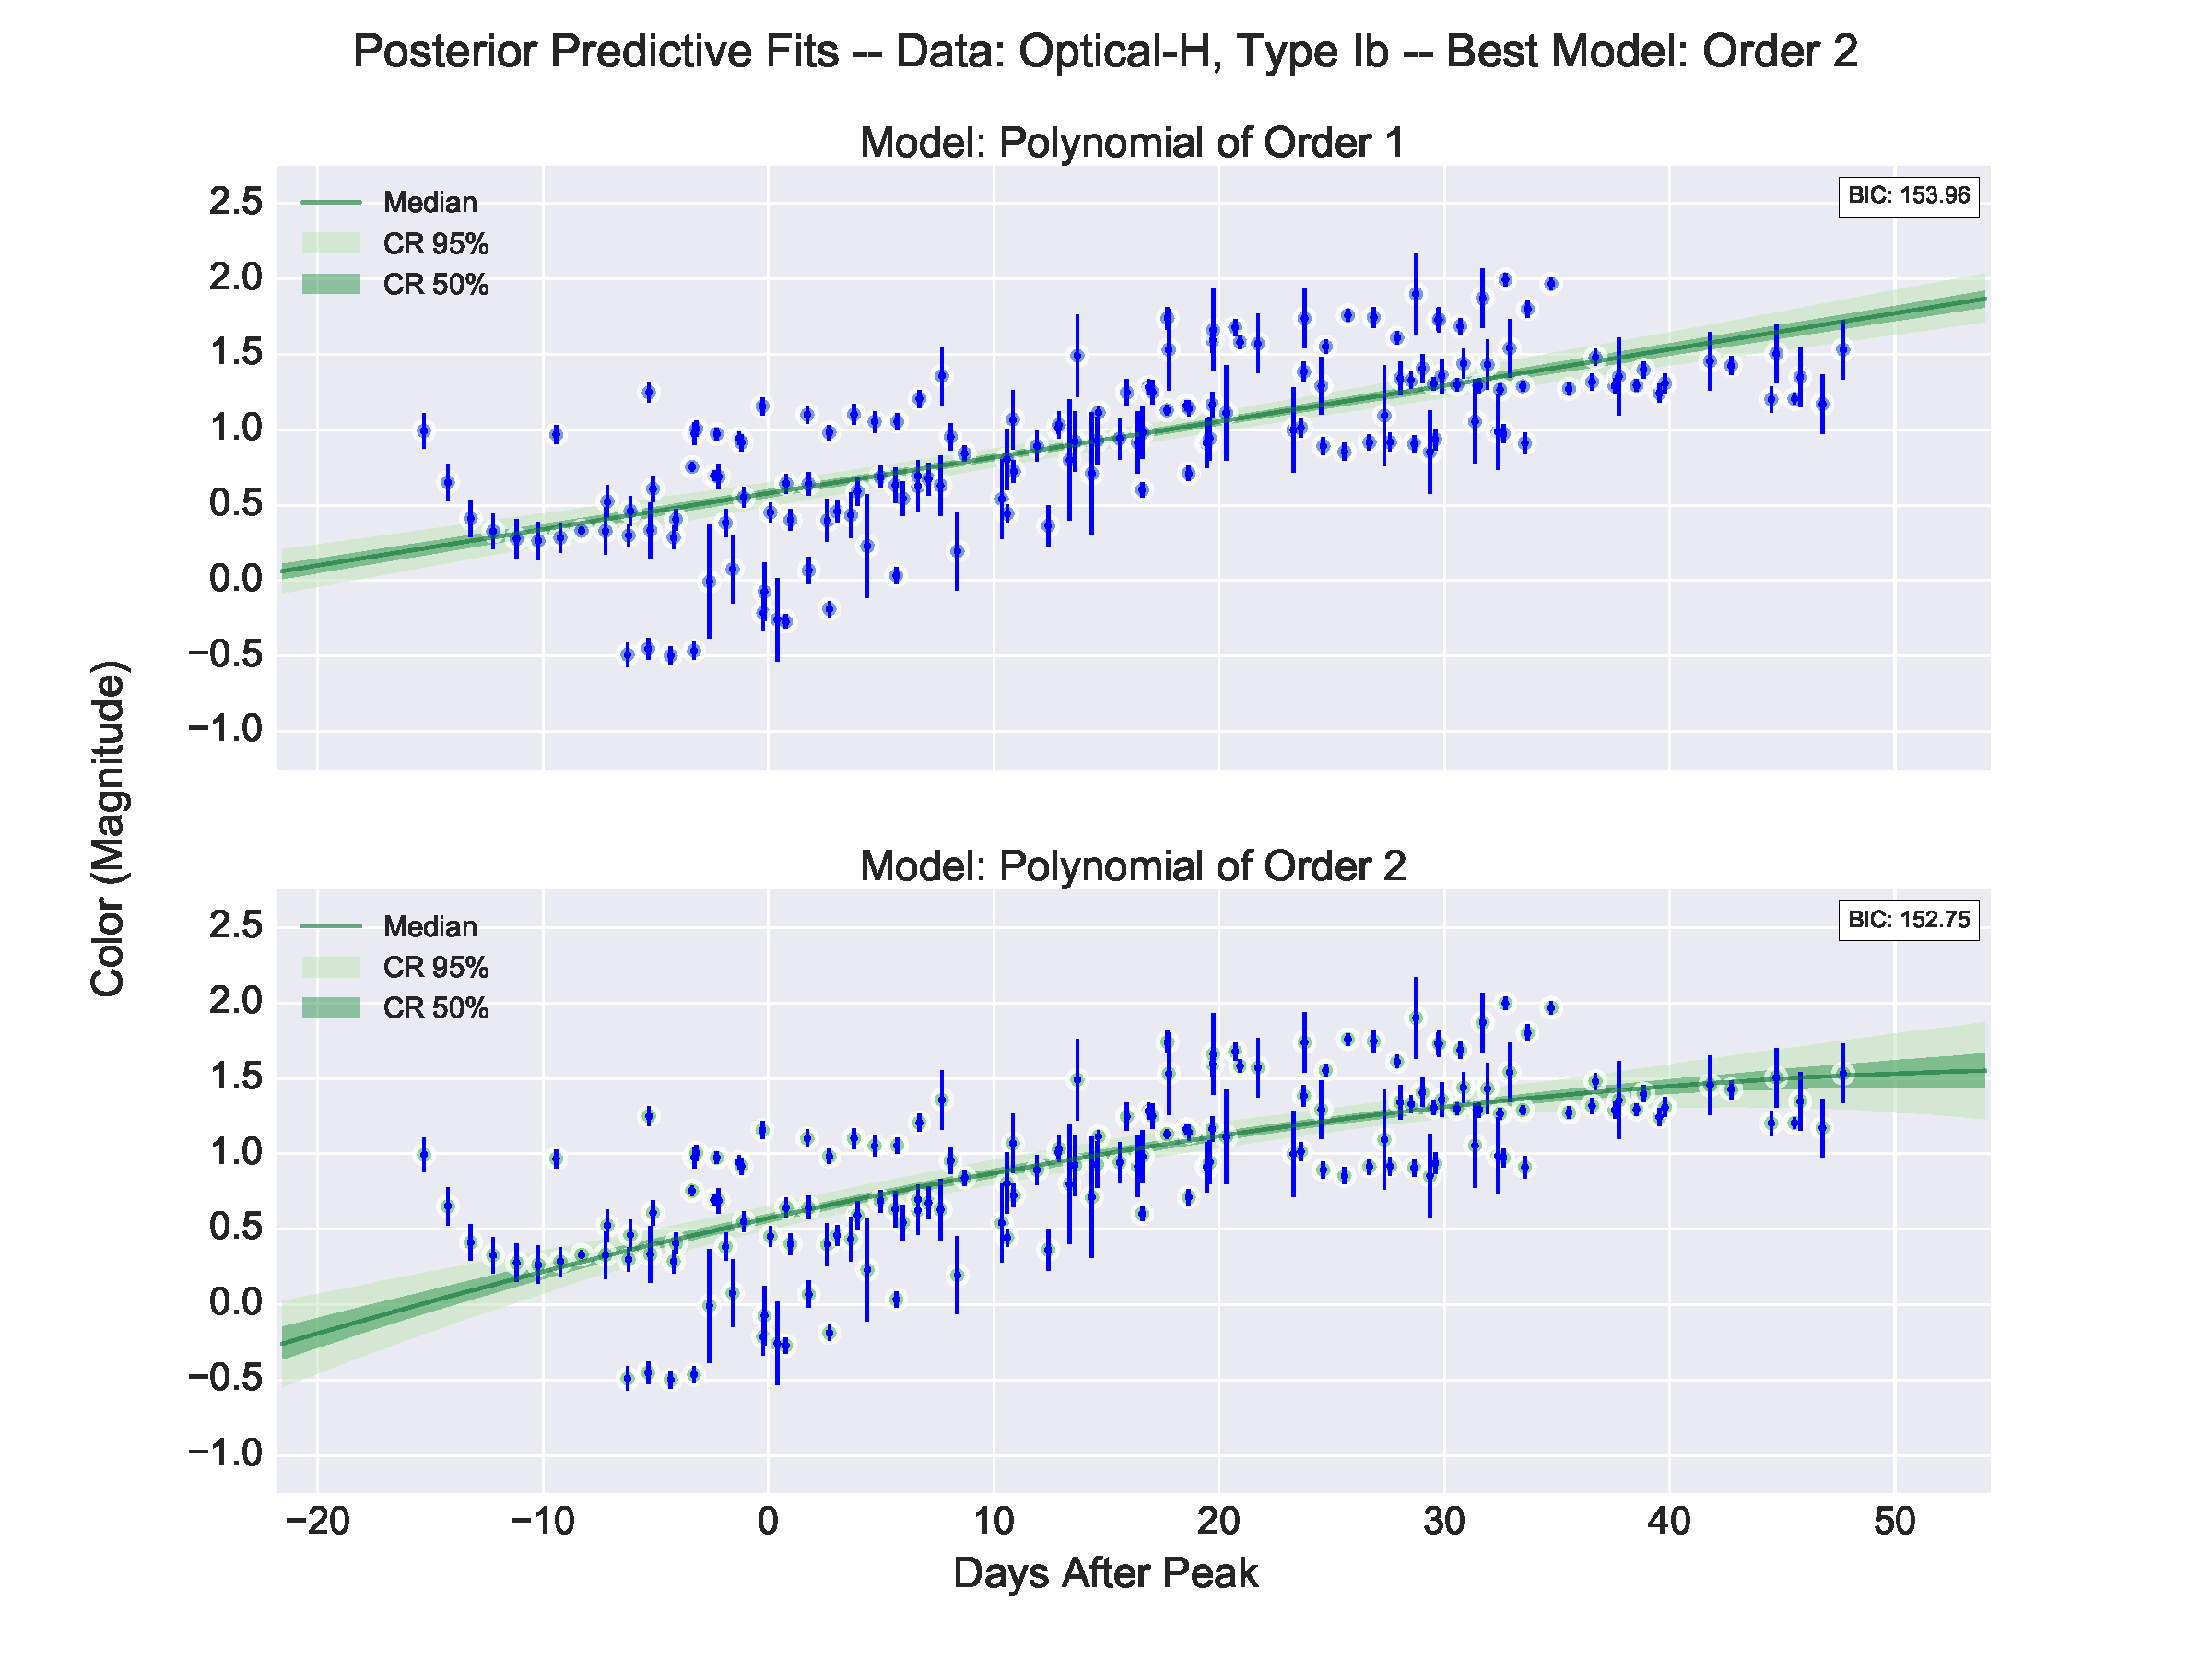
\includegraphics[scale=.5,center]{FIG/type\type/H_fits}
\end{figure}
\begin{figure}[H]
\centering
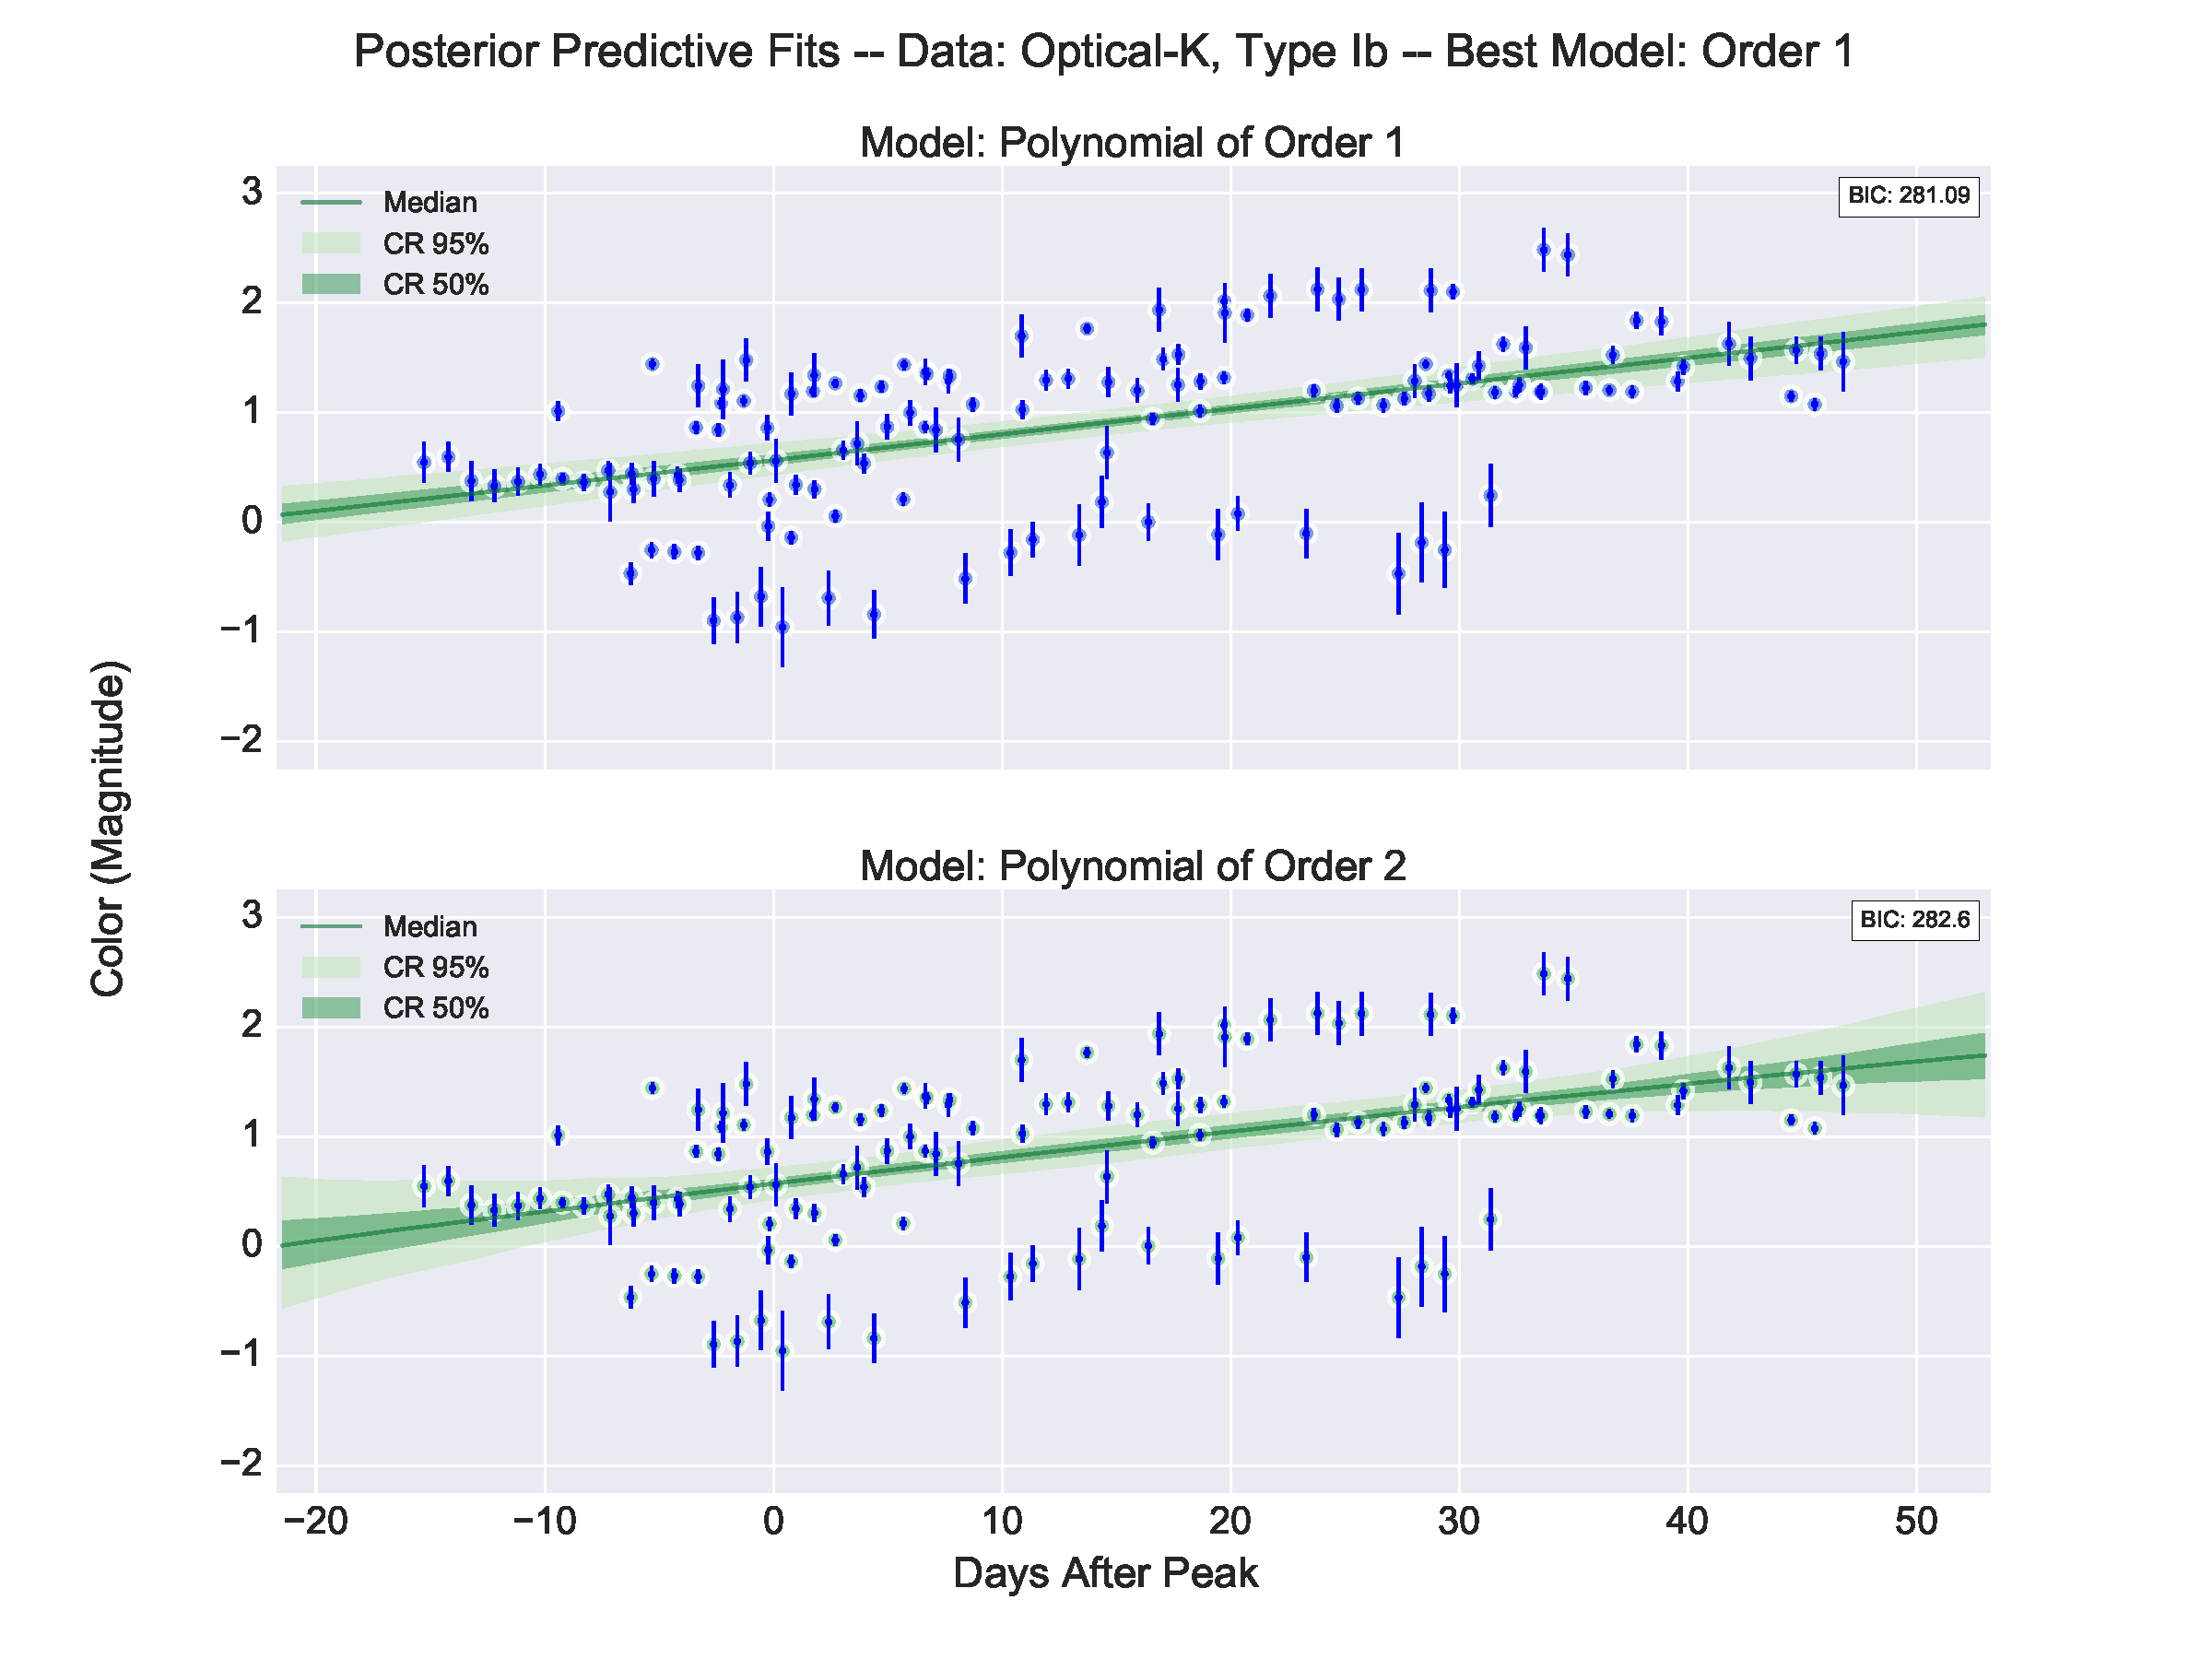
\includegraphics[scale=.5,center]{FIG/type\type/K_fits}
\end{figure}
\begin{figure}[H]
\centering
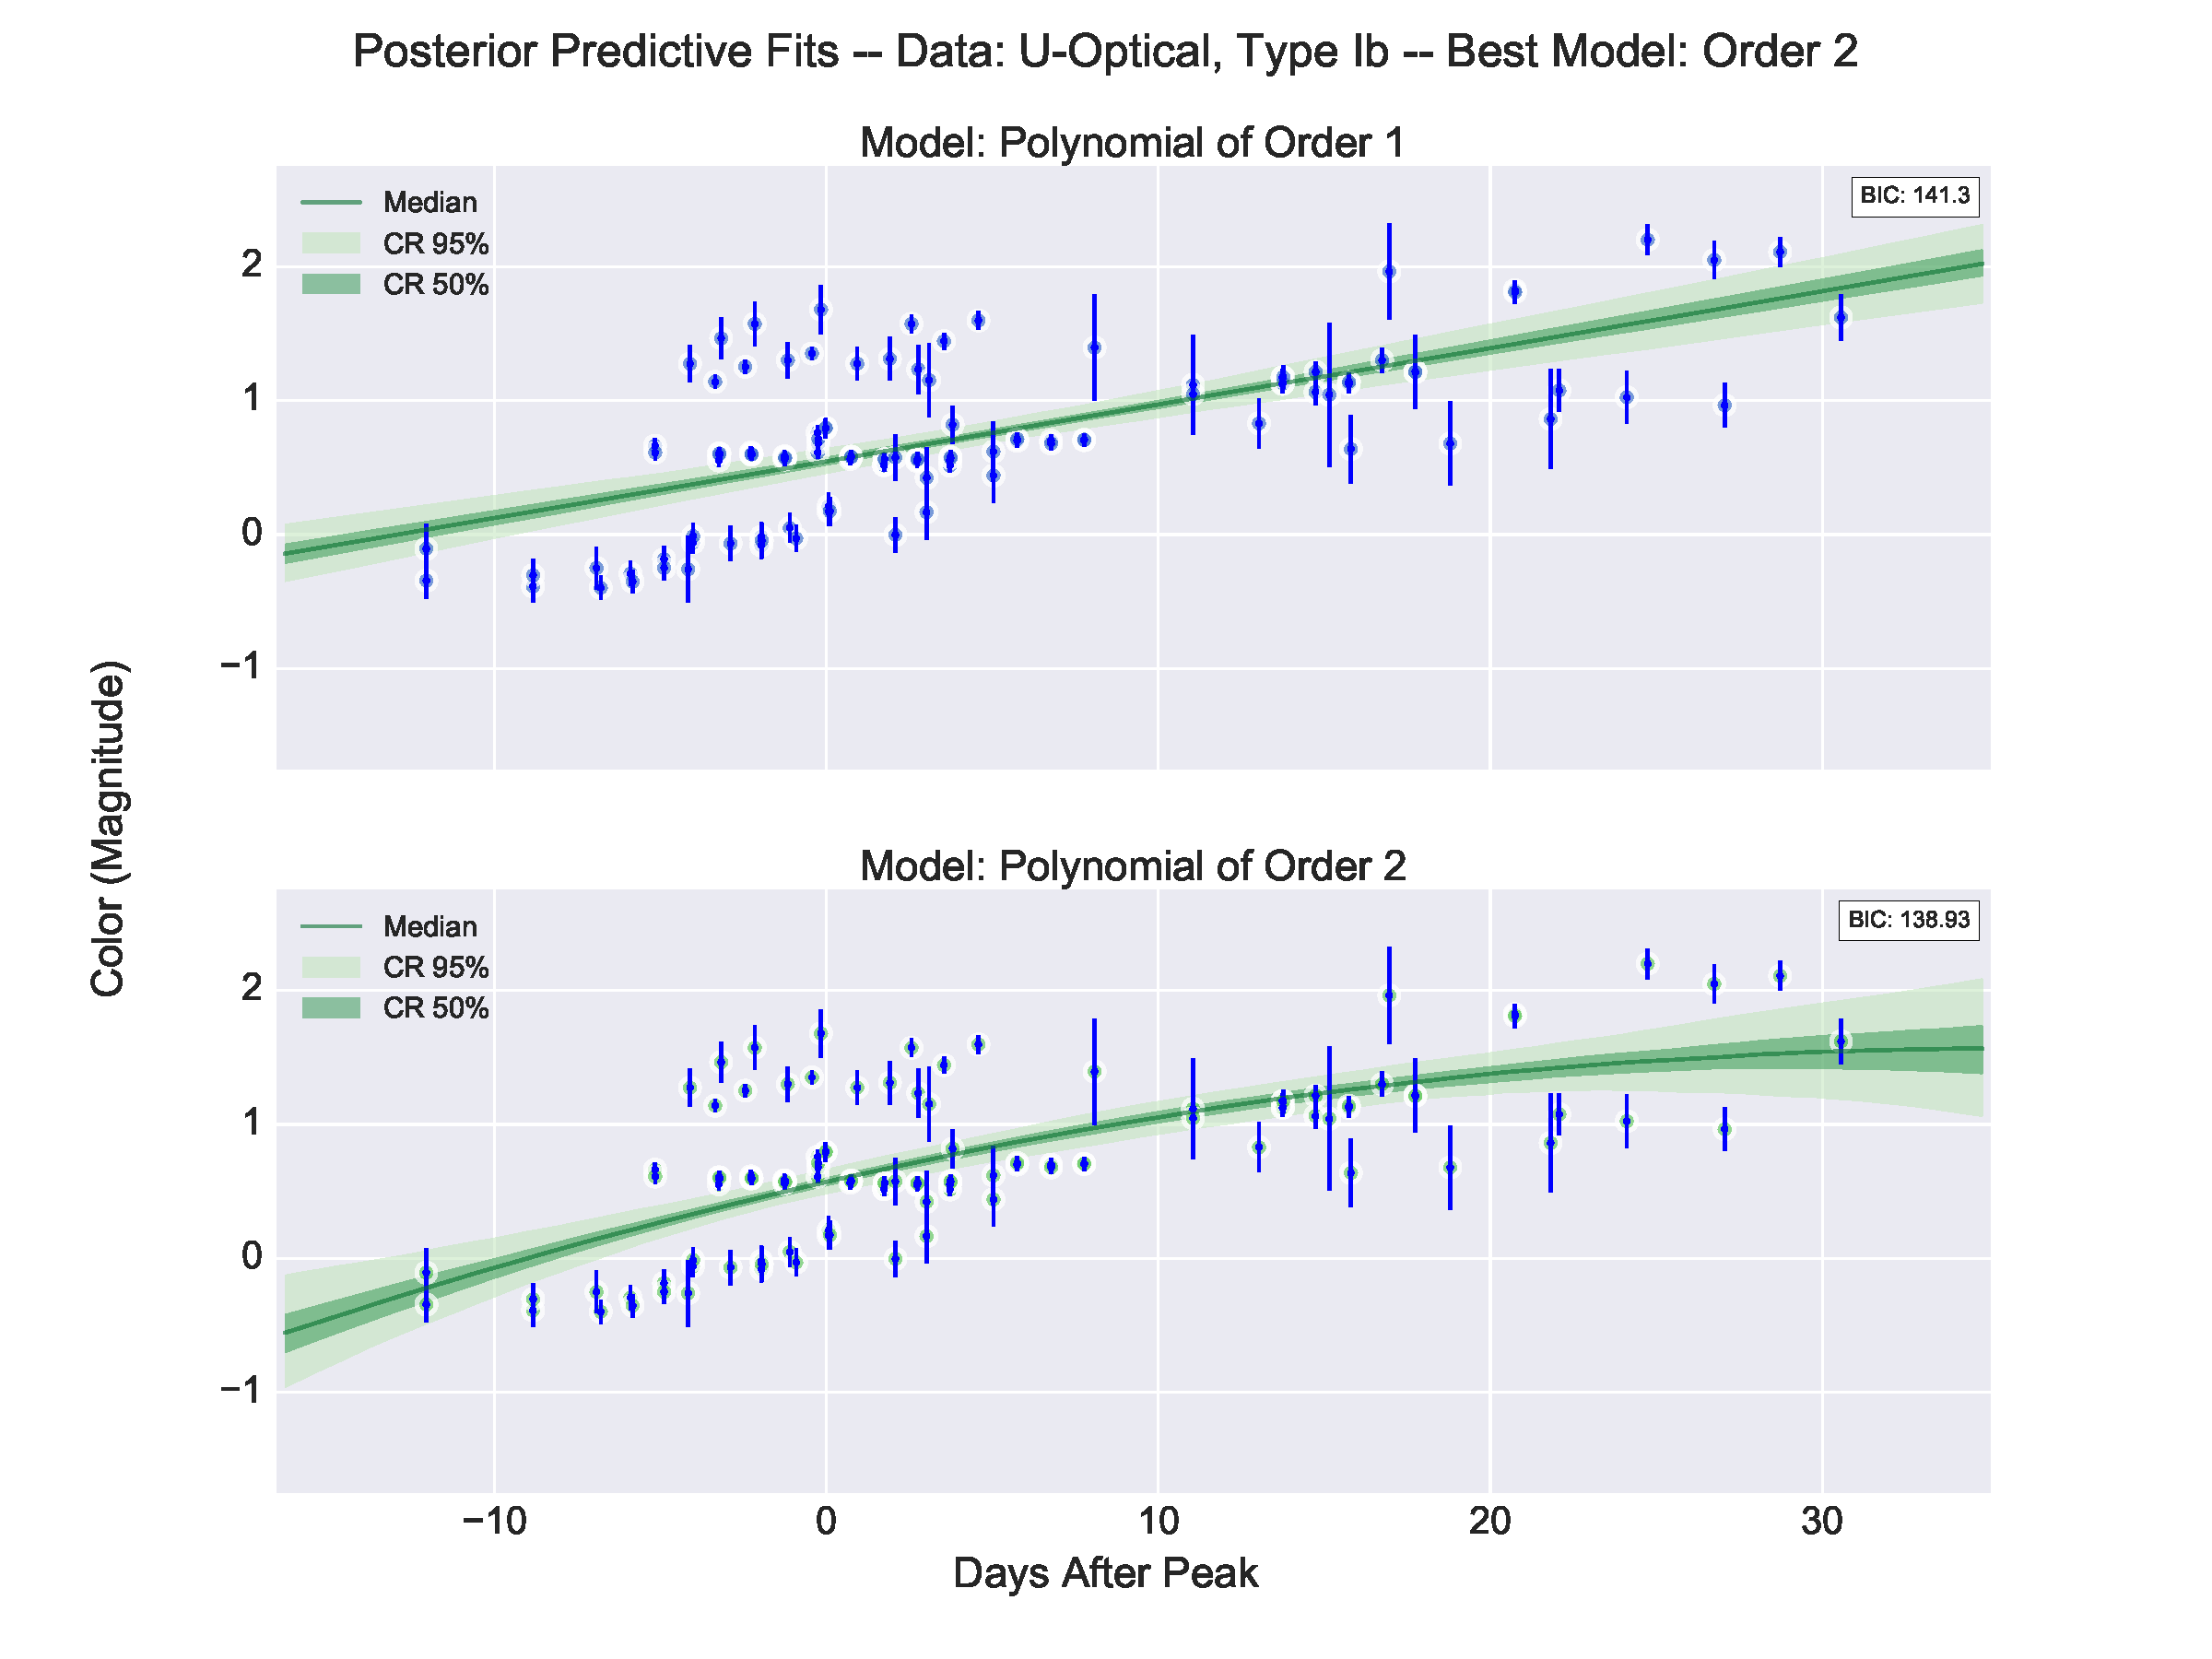
\includegraphics[scale=.5,center]{FIG/type\type/UV_fits}
\end{figure}


